\documentclass[11pt,a4paper,oldfontcommands]{memoir}
\usepackage[utf8]{inputenc}
\usepackage[T1]{fontenc}
\usepackage{microtype}
\usepackage[dvips]{graphicx}
\usepackage{xcolor}
\usepackage{times}
\usepackage[english]{babel}
\usepackage{amsthm}
\usepackage[
breaklinks=true,colorlinks=true,
%linkcolor=blue,urlcolor=blue,citecolor=blue,% PDF VIEW
linkcolor=black,urlcolor=black,citecolor=black,% PRINT
bookmarks=true,bookmarksopenlevel=2]{hyperref}

\usepackage{geometry}
% PDF VIEW
% \geometry{total={210mm,297mm},
% left=25mm,right=25mm,%
% bindingoffset=0mm, top=25mm,bottom=25mm}
% PRINT
\geometry{total={210mm,297mm},
left=20mm,right=20mm,
bindingoffset=10mm, top=25mm,bottom=25mm}

\OnehalfSpacing
%\linespread{1.3}

%%% CHAPTER'S STYLE
\chapterstyle{bianchi}
%\chapterstyle{ger}
%\chapterstyle{madsen}
%\chapterstyle{ell}
%%% STYLE OF SECTIONS, SUBSECTIONS, AND SUBSUBSECTIONS
\setsecheadstyle{\Large\bfseries\sffamily\raggedright}
\setsubsecheadstyle{\large\bfseries\sffamily\raggedright}
\setsubsubsecheadstyle{\bfseries\sffamily\raggedright}


%%% STYLE OF PAGES NUMBERING
%\pagestyle{companion}\nouppercaseheads 
%\pagestyle{headings}
%\pagestyle{Ruled}
\pagestyle{plain}
\makepagestyle{plain}
\makeevenfoot{plain}{\thepage}{}{}
\makeoddfoot{plain}{}{}{\thepage}
\makeevenhead{plain}{}{}{}
\makeoddhead{plain}{}{}{}


\maxsecnumdepth{subsection} % chapters, sections, and subsections are numbered
\maxtocdepth{subsection} % chapters, sections, and subsections are in the Table of Contents


%%%---%%%---%%%---%%%---%%%---%%%---%%%---%%%---%%%---%%%---%%%---%%%---%%%


%%%%%%%%%%%%%%From our document
%\usepackage{amsthm}

\usepackage{graphicx}
\usepackage[matrix,arrow,cmtip,curve]{xy}
\usepackage{amsmath,amssymb,hyperref}
\usepackage{tikz}
\usetikzlibrary{arrows, automata, shapes, calc, fadings}
% decorations.pathmorphing
% \usepackage{tikz-cd}
\tikzset{->, auto, >=stealth', font=\small}
\tikzset{state/.style={shape=circle, draw, fill=white, initial text=,
    inner sep=.5mm, minimum size=1.5mm}}
\tikzset{accepting/.style=accepting by arrow}
\tikzset{state with output/.style={shape=rectangle split, rectangle
    split parts=2, draw, fill=white,
    initial text=, inner sep=1mm}}



%%%%%%%%%%%%%%%%%%%%%%%%%%%%%% Tikz package
\usepackage{tikz}


%\usepackage[margin=40mm,top=35mm,bottom=35mm]{geometry}
\newcommand*\twotwo{\textsf{2+2}}
\newcommand*\down{\mathord{\downarrow}}
\newcommand*\biggdown{\mathord{\bigg\downarrow}}
\newcommand*\intord{\dashrightarrow} 
\newcommand*\evord{\intord_\ev}
\newcommand{\HDApath}{\ensuremath{$\pi$}}
\newcommand{\Dom}[1] {\mathcal{D}_{#1}}
\newcommand{\Hpath}{\mathcal{H}}
\newcommand{\HDApathIndex}[1]{\ensuremath{$\pi^{#1}$}}
\newcommand*\ev{\textup{\textsf{ev}}}
\newcommand*{\intpom}{\TrO}
\newcommand{\TrO}{\mathbf{T}}
\newcommand*\subid[3]{{}_{#1}#2_{#3}}
\newcommand*\up{\mathord{\uparrow}}
\newcommand*\exec{%
  \raisebox{1pt}{%
    \begin{tikzpicture}[x=.8ex,y=1ex,-]
      \draw (0,0) -- (1,0) -- (1,1) -- (2,1);
    \end{tikzpicture}}}
\newcommand*\ltrue{\textup{\textbf{t\!t}}}
\newcommand{\STcat}{\intpom_{\mathcal{U}}}
\newcommand*\para{\mathrel{\|}}
\newcommand*\incomp{\mathrel{\|}}
\newcommand*\rest[1]{{}_{| #1}}
\newcommand*\pobj[1]{\square^{#1}}
\newcommand*\jneda{\mathbf{j}}
%\newcommand*\intord{\dashrightarrow} 
%\newcommand*\evord{\intord_\ev}
%%%%%%%%%%%%%%%%%%%%%% For ipomset notation
\makeatother
\newcommand\pomsetwop[4]{% @R; @C; @M; content
  \vcenter{\xymatrix@1@R=#1@C=#2@M=#3{#4}}%
}
\newcommand\pomset[2][1.3]{%
  \left(%
    \pomsetwop{0ex}{#1em}{2pt}{#2}%
  \right)%
}
\newcommand\ipomset[2][1.5]{%
  \hspace*{.6em}%
  \left(%
    \hspace*{-#1em}%
    \pomsetwop{2.7ex}{#1em}{1pt}{#2}%
    \hspace*{-#1em}%
  \right)%
  \hspace*{.6em}%
}
%%%%%%%%%%%%%%
\newcommand{\ininc}{\stackrel{0}{\hookrightarrow} }
%%%%%%%%%%%%%%New theorems
%\theoremstyle{remarkstyle}\newtheorem{example}[therm]{Example}
\newtheorem{definition}{Definition}
 \newtheorem{example}[definition]{Example}
% \newdefinition{problem}{Problem}
 \newtheorem{theorem}[definition]{Theorem}
\newtheorem{conjecture}[definition]{Conjecture}
 \newtheorem{lemma}[definition]{Lemma}
 \newtheorem{proposition}[definition]{Proposition}
 \newtheorem{corollary}[definition]{Corollary}
  \newtheorem{remark}[definition]{Remark}
 %\newtheorem{proof}{Proof}
%%%%%%%%%%%%%%%%%%%%%%%%



\begin{document}

%%%---%%%---%%%---%%%---%%%---%%%---%%%---%%%---%%%---%%%---%%%---%%%---%%%
%   TITLEPAGE
%
%   due to variety of titlepage schemes it is probably better to make titlepage manually
%
%%%---%%%---%%%---%%%---%%%---%%%---%%%---%%%---%%%---%%%---%%%---%%%---%%%
\thispagestyle{empty}

{%%%
\sffamily
\centering
\Large

~\vspace{\fill}

{\huge 
Thesis title: may be long or short
}

\vspace{2.5cm}

{\LARGE
Safa Zouari
}

\vspace{3.5cm}

A thesis submitted in partial fulfillment for the\\
degree of Doctor of Philosophy\\[1em]
in the\\[1em]
Faculty Name\\
University Name

\vspace{3.5cm}

%Supervisor: Stephen Uli Fahrenberg and Krzysztof Ziemianski

\vspace{\fill}

November 2023

%%%
}%%%

\cleardoublepage
%%%---%%%---%%%---%%%---%%%---%%%---%%%---%%%---%%%---%%%---%%%---%%%---%%%
%%%---%%%---%%%---%%%---%%%---%%%---%%%---%%%---%%%---%%%---%%%---%%%---%%%

\tableofcontents*

\clearpage

%%%---%%%---%%%---%%%---%%%---%%%---%%%---%%%---%%%---%%%---%%%---%%%---%%%
%%%---%%%---%%%---%%%---%%%---%%%---%%%---%%%---%%%---%%%---%%%---%%%---%%%

\chapter{A branching time spectrum for concurrent bisimulations}

\begin{abstract}
 Higher-dimensional automata (HDAs) are models of non-interleaving concurrency for analyzing concurrent systems. HDAs subsume the main models of concurrency proposed in the literature including Petri nets, event structures, and standard automata. There is a rich literature that deals with equivalence relations for concurrent systems. Some of them have been extended to HDA. However, the logic counterpart of bisimilarity has not been widely investigated for HDAs. 
In this work, we introduce a Hennessy-Milner logic over HDAs and show that it characterizes $\mathcal{U}$-bisimulation, a branching-time bisimulation existing in the literature. In addition, we define a novel notion of bisimulation. To this end, we use the well-known notion of open map bisimulation of Joyal, Nielson, and Winskel. We rely on the categorical definition of HDAs as presheaves. Finally, we establish a comparative relation in terms of expressiveness for all variants of the notions of equivalence in question. 
\end{abstract}
%\keywords{Higher Dimensional Automata \and Hennessy-Milner logic \and Bisimulation \and Open map \and Pomsets.
%.}
\section{Introduction}
Higher Dimensional Automata (HDA), introduced by Pratt \cite{PrattCG} and van Glabbeek \cite{VANGLABBEEK2006265}, is a powerful model for non-interleaving concurrency. Van Glabbeek has placed HDA at the top of a hierarchy of concurrency models, demonstrating how other concurrency models, such as Petri nets \cite{nielsen1981petri}, configuration structure \cite{van1995configuration}, asynchronous systems \cite{bednarczyk1989categories,shields1985concurrent}, and event structure \cite{winskel1986event,winskel1989introduction}, can be incorporated into HDA \cite{VANGLABBEEK2006265}. As its name implies, a Higher Dimensional Automaton consists of a collection of $n$-dimensional hypercubes or $n$-cells connected via source and target maps. The well-known automata or labeled transition systems are obtained from the 1-dimensional objects of an HDA. However, HDAs allow for more expressive modeling of concurrent and distributed systems.
For instance, concurrent execution of two events $a$ and $b$ can be modeled by the surface of a square labeled as in Fig \ref{fi:int-conc}, while an empty square represents mutual exclusion. Analogously, a filled-in 3-dimensional cube in an HDA can represent three events $a_1,a_2,$ and $a_3$ that execute concurrently, while when considering a hollow cube, each 2-dimensional face can model $a_i \parallel a_j$ for $1 \leq i\neq j \leq 3$. 
%%%%%%%%%%%%%%%%%%%%%%%%%%%%
 \begin{figure}
    \centering
    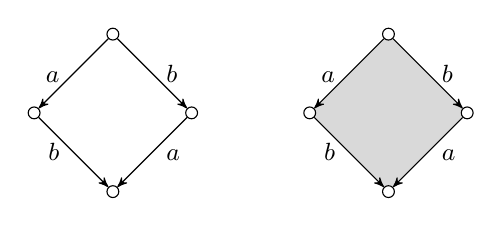
\begin{tikzpicture}[x=1cm, y=1cm]
      \begin{scope}
          \node[state] (00) at (0,0) {};
      \node[state] (10) at (-1,-1) {};
      \node[state] (01) at (1,-1) {};
      \node[state] (11) at (0,-2) {};
      \path (00) edge node[left] {$\vphantom{b}a$\,} (10);
      \path (00) edge node[right] {\,$b$} (01);
      \path (10) edge node[left] {$b$\,} (11);
      \path (01) edge node[right] {\,$\vphantom{b}a$} (11);
      \end{scope}
      \begin{scope}[shift={(3.5,0)}]
         \path[fill=black!15] (0,0) to (-1,-1) to (0,-2) to (1,-1);
      \node[state] (00) at (0,0) {};
      \node[state] (10) at (-1,-1) {};
      \node[state] (01) at (1,-1) {};
      \node[state] (11) at (0,-2) {};
      \path (00) edge node[left] {$\vphantom{b}a$\,} (10);
      \path (00) edge node[right] {\,$b$} (01);
      \path (10) edge node[left] {$b$\,} (11);
      \path (01) edge node[right] {\,$\vphantom{b}a$} (11);
      \end{scope}
    \end{tikzpicture}
    \bigskip
     \caption{HDA models distinguishing interleaving $a. b+ b. a$ (left) from non-interleaving concurrency $a\para b$ (right).}
  \label{fi:int-conc}
  \end{figure}

Formally, a higher-dimensional automaton is a specific precubical set, equipped with a set of initial cells and a set of final cells. Like a simplicial set, a precubical set is built up out of gluing hypercubes to each other in a consistent manner. More precisely, a precubical set is a graded set $X= \bigcup_{n \in \mathbf{N}}X_n$, where $X_n$ is the set of $n$-cells equipped with elementary face maps $\delta_{ i, n}^\nu:  X_n\to X_{ n- 1}$ that map an $n$-cell to its face. The choice of the face is determined by $i\in\{ 1,\dotsc, n\}$ and $\nu\in\{ 0, 1\}$ and respects the following precubical identity.
\begin{equation*}
  \delta_{ i, n- 1}^\nu \delta_{ j, n}^\mu= \delta_{ j- 1, n- 1}^\mu
  \delta_{ i, n}^\nu,
\end{equation*}
See Fig \ref{fi:2cubefaces-full} for an example where the precubical identity can be verified at the corners of the square $x$.% Each $n$-cell is associated with a linearly ordered and labeled set $V$ of length $n$. From a concurrency point of view, such a cell models a list $V$ of $n$ active events. A lower face of a cell $x_n \in X_n$ is a cell that has $U \subseteq V$ as active events. For example, in Fig. \ref{fi:int-conc}, the square has active events $[a b]$. Its faces have active events $[a]$ and $[b]$, respectively. In Section \ref{sec:HDA}, we make this precise by defining precubical sets as presheaves over a category of linearly ordered sets with appropriate morphisms \cite{LanguageofHDA,KleeneTh}.

In addition to concurrency models, equivalence relations should also be considered when describing concurrent systems. This is because these models might not be abstract enough. To address this, various notions of equivalence have been suggested in studies \cite{sangiorgi1998bisimulation,van2001refinement,vanGlabbeek1997difference,gorrieri2021team,leifer2000deriving,abramsky2021relating,Uli14}, guided by considerations of the critical aspects of system behavior within a specific context and the elements from which to abstract. Parallel to behavioral equivalences, modal logic is a useful formalism for specifying and verifying properties of concurrent systems \cite{aceto2007reactive,de1989linear,pnueli1992temporal,baier2008principles,baldan2020model}. Characterization of bisimulation in terms of Hennesey-Milner logic (HML) provides additional confidence in both approaches: Two systems are bisimilar iff they satisfy the same logical assertions. The literature focusing on logical characterization includes Van Glabbek spectrum \cite{Van.br} for sequential process and \cite{baldan2010logic,nielsen1994bisimulation,de1995three,nielsen2005bisimulation,phillips2014event,baldan2014hereditary} for concurrent systems. Some of these behavioral equivalences have been extended to HDA. Among them are hereditary history-preserving bisimulations (hh-bisimulation) and ST-bisimulations \cite{VANGLABBEEK2006265}. However, to the best of our knowledge, their logical counterpart has not been investigated for HDA.

This paper presents a variant of (HML) interpreted over HDA. The original HML in the interleaving setting \cite{hennessy1985algebraic}, contains negation $(\neg )$, conjunction $(\wedge)$, a formula $\top$ that always holds, and a diamond modality $\langle a \rangle F$, which says that it is possible to perform an action labeled by $a$ and reach a state that satisfies $F$. Unlike the standard HML, our logic considers both sequential and concurrent computations. Thus, it differs from the standard HML within the diamond modality so that it becomes $\langle P \rangle F$ where $P$ is a pomset (interval with interfaces) and interpreted over a path $\alpha$, which says that there is a path $\beta$ labeled by $P$ that extends $\alpha$ to a path (concatenation of $\alpha$ and $\beta$) that satisfies $F$. For example, in Fig. \ref{fi:2cubefaces-full}, the formula $\langle (a \longrightarrow b) \rangle \top \vee \langle (b \longrightarrow a) \rangle \top$, which stands for mutual exclusion, holds at the top edge of both squares. While the formula $\langle \pomset{a \\ c} \rangle \top$ holds only on the top corner of the filled-in square (on the right). The latter formula shows that our logic is powerful enough to distinguish interleaving from true concurrency. 

Pomsets were first introduced by Winkowski \cite{winkowski1977algebraic}. Interval orders, a subclass of pomsets, have been introduced by Fishburn \cite{fishburn1970intransitive}. Uli et al. \cite{LanguageofHDA} extended the concept of (interval) pomsets with interfaces, facilitating the definition of the gluing composition of HDA languages.
 A computational run in an HDA is modeled by a path, a sequence of cells. Each two consecutive cells are related by a source or a target map. The observable contents of a path $\alpha$ are described by $\ev(\alpha)$, an interval pomset equipped with interfaces. Fig \ref{fi:hda-a|cd-dpaths} shows 3 examples of paths with their corresponding pomsets (below).

%We show that the resulting logic is characteristic of a variant of ST-bisimulation, the $\mathcal{U}$-bisimulation. When equipped with backward modality, it characterized the strong $\mathcal{U}$-bisimulation


 % we stopped here

%To keep our paper self-contained, we recall the definition and the properties of ipomsets in Section \ref{subsec: ipomset}. 

\begin{figure}
  \centering
  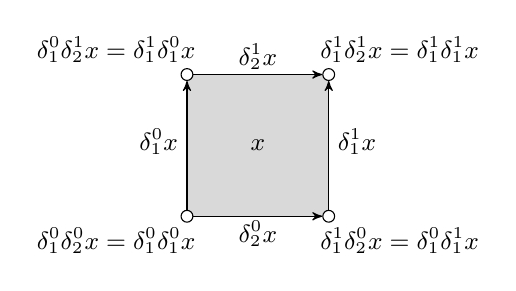
\begin{tikzpicture}[x=.9cm,y=.9cm]
    \path[fill=black!15] (0,0) to (2,0) to (2,2) to (0,2) to (0,0);
    \node[state] (00) at (0,0) {};
    \node[state] (10) at (2,0) {};
    \node[state] (01) at (0,2) {};
    \node[state] (11) at (2,2) {};
    \path (00) edge (01);
    \path (00) edge (10);
    \path (01) edge (11);
    \path (10) edge (11);
    \node at (1,1) {$x$};
    \node at (-.4,1.05) {$\delta_1^0 x$};
    \node at (2.4,1.05) {$\delta_1^1 x$};
    \node at (1,-.25) {$\delta_2^0 x$};
    \node at (1,2.25) {$\delta_2^1 x$};
    \node at (-1,-.35) {$\delta_1^0 \delta_2^0 x= \delta_1^0
      \delta_1^0 x$};
    \node at (-1,2.35) {$\delta_1^0 \delta_2^1 x= \delta_1^1
      \delta_1^0 x$};
    \node at (3,-.35) {$\delta_1^1 \delta_2^0 x= \delta_1^0
      \delta_1^1 x$};
    \node at (3,2.35) {$\delta_1^1 \delta_2^1 x= \delta_1^1
      \delta_1^1 x$};
  \end{tikzpicture}
  \bigskip
  \caption{%
    \label{fi:2cubefaces-full} (\cite{LanguageofHDA})
    A square $x$ with its four elementary faces $\delta_1^0 x$,
    $\delta_1^1 x$, $\delta_2^0 x$, $\delta_2^1 x$ and four corners.
  }
\end{figure}

%Partial words and pomsets has been introduced by Winkowski \cite{winkowski1977algebraic} and hold a longstanding role as semantics in concurrent systems \cite{PrattCG,vogler1992modular}. Interval orders, a subclass of pomsets,  have been introduced by Fishburn \cite{fishburn1970intransitive} and are extensively used in concurrency theory and distributed systems. Uli et al. \cite{LanguageofHDA} extended the concept of (interval) pomsets with interfaces, facilitating the definition of the gluing composition of HDA languages. Figure \ref{fi:hda-a|cd-dpaths} provides illustrative examples of interval pomsets. This work relied heavily on the definition of interval pomset with interfaces (iipomset).
%Different concurrency models exist with different notions of equivalence, complicating understanding their differences. Using a category-theoretic approach, these models can be clarified and unified through the category of models \cite{winskel1995m}. 

To define the notion of bisimulation and the path logic over HDA, we employ the well-known notion of open map bisimulation \cite{JOYAL1996164}. This approach requires a category of model $\mathbf{M}$ (the category of HDA in our case) and a category of paths $\TrO$, a small subcategory of $\mathbf{M}$ (a category of track objects in our case). Track objects have originally been introduced in \cite{LanguageofHDA} to define the language of HDA. They form a subcategory of $\mathbf{M}$. A track object is a particular HDA that can be constructed from a given iipomset $P$, denoted $\square^P$. For instance, in Fig \ref{fi:hda-a|cd-dpaths}, each track object in the second line is constructed from the iipomset above it. Intuitively, for a given path $\pi$ labeled with an iipomset $P$, a track object $\square^P$ is the smallest HDA containing $\pi$. See also Fig. \ref{fi:hda-a|cd-dpaths}. We show that the resulting logic characterizes $\mathcal{U}$-bisimulation. However, its extension, equipped with backward modality characterizes the strong $\mathcal{U}$-bisimulation. Finally, we finish this paper with a hierarchy of the equivalence relations encountered in the paper. Other contributions that deepen the understanding of the mathematical structure used and may be independent of interest include showing that track objects and iipomsets define the same objects, a relation between the notion of paths of Van Glabbeek \cite{VANGLABBEEK2006265} and track of Uli et al. \cite{LanguageofHDA}, and a generalization of the Yoneda lemma.
 
\begin{figure}
  \centering
  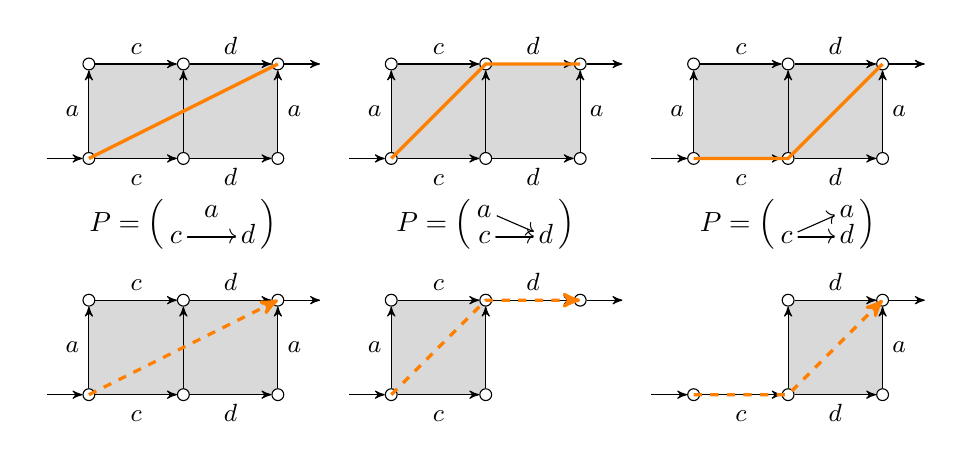
\begin{tikzpicture}[x=1.2cm, y=1.2cm]
    \begin{scope}
      \path[fill=black!15] (0,0) to (2,0) to (2,1) to (1,1) to
      (0,1);
      \node[state, initial] (00) at (0,0) {};
      \node[state] (10) at (1,0) {};
      \node[state] (20) at (2,0) {};
      \node[state] (01) at (0,1) {};
      \node[state] (11) at (1,1) {};
      \node[state, accepting] (21) at (2,1) {};
      \path (00) edge node[below] {$\vphantom{d}c$} (10);
      \path (10) edge node[below] {$d$} (20);
      \path (01) edge node[above] {$c$} (11);
      \path (11) edge node[above] {$d$} (21);
      \path (00) edge node[left] {$a$} (01);
      \path (10) edge (11);
      \path (20) edge node[right] {$a$} (21);
      \draw[-, very thick, orange] (0,0) -- (2,1);
     \node[font=\normalsize] at (1,-.7) {$P=\pomset[.4]{ & a \\ c
          \ar[rr] && d}$};
        %   \node[font=\normalsize] at (-.35,0.2) {$i$};
    \end{scope}
    \begin{scope}[shift={(3.2,0)}]
      \path[fill=black!15] (0,0) to (2,0) to (2,1) to (1,1) to
      (0,1);
      \node[state, initial] (00) at (0,0) {};
      \node[state] (10) at (1,0) {};
      \node[state] (20) at (2,0) {};
      \node[state] (01) at (0,1) {};
      \node[state] (11) at (1,1) {};
      \node[state, accepting] (21) at (2,1) {};
      \path (00) edge node[below] {$\vphantom{d}c$} (10);
      \path (10) edge node[below] {$d$} (20);
      \path (01) edge node[above] {$c$} (11);
      \path (11) edge node[above] {$d$} (21);
      \path (00) edge node[left] {$a$} (01);
      \path (10) edge (11);
      \path (20) edge node[right] {$a$} (21);
      \draw[-, very thick, orange] (0,0) -- (1,1) -- (2,1);
    \node[font=\normalsize] at (1,-.7) {$P=\pomset{a\ar[dr] \\ c\ar[r] & d}$};
    % \node[font=\normalsize] at (-.35,0.2) {$i$};
    \end{scope}
    \begin{scope}[shift={(6.4,0)}]
      \path[fill=black!15] (0,0) to (2,0) to (2,1) to (1,1) to
      (0,1);
      \node[state, initial] (00) at (0,0) {};
      \node[state] (10) at (1,0) {};
      \node[state] (20) at (2,0) {};
      \node[state] (01) at (0,1) {};
      \node[state] (11) at (1,1) {};
      \node[state, accepting] (21) at (2,1) {};
      \path (00) edge node[below] {$\vphantom{d}c$} (10);
      \path (10) edge node[below] {$d$} (20);
      \path (01) edge node[above] {$c$} (11);
      \path (11) edge node[above] {$d$} (21);
      \path (00) edge node[left] {$a$} (01);
      \path (10) edge (11);
      \path (20) edge node[right] {$a$} (21);
      \draw[-, very thick, orange] (0,0) -- (1,0) -- (2,1);
    \node[font=\normalsize] at (1,-.7) {$P=\pomset{ & a \\ c\ar[r]\ar[ur] & d}$};
  %   \node[font=\normalsize] at (-.35,0.2) {$i$};
    \end{scope}
    \begin{scope}[shift={(0,-2.5)}]
     \begin{scope}
      \path[fill=black!15] (0,0) to (2,0) to (2,1) to (1,1) to
      (0,1);
      \node[state, initial] (00) at (0,0) {};
      \node[state] (10) at (1,0) {};
      \node[state] (20) at (2,0) {};
      \node[state] (01) at (0,1) {};
      \node[state] (11) at (1,1) {};
      \node[state, accepting] (21) at (2,1) {};
      \path (00) edge node[below] {$\vphantom{d}c$} (10);
      \path (10) edge node[below] {$d$} (20);
      \path (01) edge node[above] {$c$} (11);
      \path (11) edge node[above] {$d$} (21);
      \path (00) edge node[left] {$a$} (01);
      \path (10) edge (11);
      \path (20) edge node[right] {$a$} (21);
      \draw[dashed, very thick, orange] (0,0) -- (2,1);
      %\node[font=\normalsize] at (1,-.7) {$\pomset[.4]{ & a \\ c
       %   \ar[rr] && d}$};
    \end{scope}
    \begin{scope}[shift={(3.2,0)}]
      \path[fill=black!15] (0,0) to (1,0) to (1,1)  to
      (0,1);
      \node[state, initial] (00) at (0,0) {};
      \node[state] (10) at (1,0) {};
   %   \node[state] (20) at (2,0) {};
      \node[state] (01) at (0,1) {};
      \node[state] (11) at (1,1) {};
      \node[state, accepting] (21) at (2,1) {};
      \path (00) edge node[below] {$\vphantom{d}c$} (10);
      %\path (10) edge node[below] {$d$} (20);
      \path (01) edge node[above] {$c$} (11);
      \path (11) edge node[above] {$d$} (21);
      \path (00) edge node[left] {$a$} (01);
      \path (10) edge (11);
      %\path (20) edge node[right] {$a$} (21);
      % \draw[-, path fading=west] (0,0) -- (-.3,0);
      \draw[dashed, very thick, orange] (0,0) -- (1,1) -- (2,1);
     %\node[font=\normalsize] at (1,-.7) {$\pomset{a\ar[dr] \\ c\ar[r] & d}$};
    \end{scope}
    \begin{scope}[shift={(6.4,0)}]
     \path[fill=black!15] (1,0) to (2,0) to (2,1) to (1,1) ;
      \node[state, initial] (00) at (0,0) {};
      \node[state] (10) at (1,0) {};
      \node[state] (20) at (2,0) {};
    %  \node[state] (01) at (0,1) {};
      \node[state] (11) at (1,1) {};
      \node[state, accepting] (21) at (2,1) {};
      \path (00) edge node[below] {$\vphantom{d}c$} (10);
      \path (10) edge node[below] {$d$} (20);
      %\path (01) edge node[above] {$c$} (11);
      \path (11) edge node[above] {$d$} (21);
      %\path (00) edge node[left] {$a$} (01);
      \path (10) edge (11);
      \path (20) edge node[right] {$a$} (21);
      \draw[dashed, very thick, orange!] (0,0) -- (1,0) -- (2,1);
    %\node[font=\normalsize] at (1,-.7) {$\pomset{ & a \\ c\ar[r]\ar[ur] & d}$};
    \end{scope}
   \end{scope}
  \end{tikzpicture}
  \smallskip
  \caption{Paths in an HDA (First line) together
    with corresponding track objects (second line) \cite{LanguageofHDA}.}
  \label{fi:hda-a|cd-dpaths}
\end{figure}



\section{Higher Dimensional Automata}\label{sec:HDA}
We review the definition of Higher Dimensional Automata. We rely on a categorical approach proposed and studied by Uli at el \cite{LanguageofHDA, KleeneTh}, where HDA is defined as a specific precubical 


To define precubical sets as presheaves over the labeled precube category $\boxdot$, we introduce conclists, the objects of $\boxdot$ and coface maps, and the morphisms of $\boxdot$.

\begin{definition}{(Conclists)}
A concurrency list or conclist is a tuple $(U, \dashrightarrow, \lambda)$, where $U$ is a finite set totally ordered by the strict order $\dashrightarrow$ and $\lambda: U \rightarrow \Sigma $ is a labeling map. Elements of $U$ will be called events. A conclist-map is a label and order-preserving map between conclists. 
\end{definition}
 As the order $\dashrightarrow$ is strict and total, all conclist-maps are injective. Each conclist-map $f: U \rightarrow V$ defines and is uniquely defined by $A= V \setminus f(U)$, such a map will be denoted by $f_A: U\to V$. We write $U\simeq V$ if there exists a surjective conclist map $f_A$ between them. If such an isomorphism exists then it is unique, since $f_A$ is surjective iff $A=\emptyset$.  
\begin{definition}{(Coface maps)}
    A coface map $d_{A, B}: U \to V$ is a tuple $(f_{A \cup B}, A, B)$ where $f_{A \cup B}: U \to V$ is a conclist map and $A \cap B = \emptyset$. The tuple \linebreak $\bigl(f_{C \cup D} \circ f_{A\cup B},f_{C \cup D}(A) \cup C, f_{C \cup D}(B)\cup D \bigl)$ defines $d_{C,D}\circ d_{A,B} : U \rightarrow W$, the composite of $d_{A,B}: U \rightarrow V$ and $d_{C,D}: V \rightarrow W$ and is a coface map, as the sets $f_{C \cup D}(A), C, f_{C \cup D}(B), D \subseteq W$ are pairwise disjoint. In addition, we have $W \setminus  f_{C\cup D}\circ f_{A\cup B}(U) = f_{C\cup D}(A) \cup f_{C\cup D}(B) \cup C \cup D.$ %This can be shown by the elementary calculation.
\end{definition} %\begin{align*}
 %& V=f_{A\cup B}(U) \cup A \cup B, \text{ thus } f_{C\cup D}(V)=f_{C\cup D}\circ f_{A\cup B}(U) \cup f_{C\cup D}(A) \cup f_{C\cup D}(B).\\
 %& \text{Since } W \setminus f_{C\cup D}(V)= C \cup D, W \setminus \bigl(  f_{C\cup D}\circ f_{A\cup B}(U) \cup f_{C\cup D}(A) \cup f_{C\cup D}(B) \bigl)=C \cup D,\\
 %& \text{thus } W \setminus  f_{C\cup D}\circ f_{A\cup B}(U) = f_{C\cup D}(A) \cup f_{C\cup D}(B) \cup C \cup D.
%\end{align*}
Intuitively, a coface map $d_{A, B}: U \rightarrow V$ identifies events of $U$ with events $f_{A \cup B}(U)$ of $V$ and splits $V \setminus f_{A \cup B}(U)$ into two disjoint subsets: $A\subseteq V$ for unstarted events in $U$ and $B\subseteq V$ for terminated events in $U$. Conclists together with coface maps as morphisms form the precube category $\boxdot$ introduced in \cite{KleeneTh}. Another alternative approach, proposed in \cite{LanguageofHDA}, will be discussed subsequently.

To define the labeled precube category, we only need particular compositions of morphisms  $d_{A, B}: S \rightarrow T$ and $d_{C, D}: T \rightarrow U$ for pairwise disjoint $A, B, C, D \subseteq U$ and $T=U \backslash(C \cup D)$, that is $f_{C \cup D}(t)=t$ for all $t\in T$. In this case:
$$
d_{C, D} \circ d_{A, B}=d_{A \cup C, B \cup D}.
$$
%%%%%%%%%%%%%%%%%%%%%%% Our proof is correct but we will write for the general case:
For $d_{A, B}: S \rightarrow T$, $d_{C, D}: T \rightarrow U$, $d_{E, G}: U \rightarrow V$, $f_{C \cup D}(A), f_{C \cup D}(B),C, D, E, G \subseteq V$ pairwise disjoint, and $U=V \backslash(E \cup G)$,% and hence $T=V \backslash(C \cup E \cup D \cup G)$,
\begin{align*}
    ( d_{E, G} \circ d_{C, D} ) \circ d_{A, B}  & = \bigl(f_{E \cup G} \circ f_{C\cup D},f_{E \cup G}(C) \cup E, f_{E \cup G}(D)\cup G \bigl) \circ \bigl(f_{A \cup B},A,B \bigl) \\ %still under test
    & = \bigl( f_{C\cup D},C \cup E, D\cup G \bigl) \circ \bigl(f_{A \cup B},A,B \bigl) \\ %still under test
    & = \bigl( f_{C\cup D} \circ f_{A \cup B},  f_{C\cup D}(A) \cup C \cup E ,  f_{C\cup D}(B) \cup D \cup G \bigl) \\ %still under test
    & = \bigl(f_{E\cup G},E,G \bigl) \circ \bigl( f_{C\cup D} \circ f_{A \cup B},  f_{C\cup D}(A) \cup C ,  f_{C\cup D}(B) \cup D  \bigl)  \\ %still under test
    & = d_{E, G} \circ (d_{C, D}  \circ d_{A, B}),
\end{align*}
%Thus for $d_{A, B}: S \rightarrow T$, $d_{C, D}: T \rightarrow U$, and %$d_{E, G}: U \rightarrow V$ for, pairwise disjoint $A, B, C, D, E, G %\subseteq V$, $T=U \backslash(C \cup D)$, $U=V \backslash(E \cup G)$, and %hence $T=V \backslash(C \cup E \cup D \cup G)$,
%\begin{align*}
 %   ( d_{A, B} \circ d_{C, D} ) \circ d_{E, G} & = d_{A\cup C, B \cup D}  \circ d_{E, G}\\
  %  & = d_{(A\cup C)\cup E, (B \cup D) \cup G}\\
  %  & = d_{A \cup (C\cup E), B \cup (D \cup G)}\\
  %  & = d_{A, B} \circ d_{C\cup E, D \cup G}\\
  %  & = d_{A, B} \circ (d_{C, D} \circ d_{E, G}),
%\end{align*}
so that the composition of coface maps is associative. Now, we are ready to define the labeled precube category.
%%%%%%%%%%%%%%%%%%%%%%
\begin{definition}
The large labeled precube category $\boxdot$ consists of the following data:
\begin{itemize}
  \item Objects are conclists $(S,\dashrightarrow)$;
 \item Morphisms are coface maps $d_{A,B} : U\rightarrow V$. %Each $d_{A, B}$ is a triple $\left(f_{A \cup B}, A, B\right)$ with $A, B \subseteq V$ disjoint and $f_{A \cup B}: U \hookrightarrow V$ an lo-map;
  \item The composition of morphisms $d_{A, B}: U \rightarrow V$ and $d_{C, D}: V \rightarrow W$ is defined as above.
\end{itemize}
\end{definition}
We write $d_{A}^{0}$ for $d_{A, \emptyset}$, $d_{B}^{1}$ for $d_{\emptyset, B}$, $\mathbf{id}^{\boxdot}_{U}$ for the identity morphism $d_{\emptyset, \emptyset}: U \rightarrow U$.
The second approach to defining the labeled precube category has been introduced in \cite{LanguageofHDA}, where objects are the same as $\boxdot$ but with different morphisms, defined as follows.
\begin{definition}\label{def: precube} 
Let $\square$ be the category formed by conclists as objects and morphisms between conclists $U$ and $V$ generated by $(f,\varepsilon)$ where $f: U \rightarrow V$ is a conclist-map and $\varepsilon: T\rightarrow \{ 0,\exec, 1 \}$ such that $\varepsilon^{-1}(\exec)= f(U)$. The composition of morphisms $(f,\varepsilon):S\to T$ and
    $(g,\zeta):T\to U$ is $\bigl((g,\zeta) \circ (f,\varepsilon)  \bigl)=(g\circ f,\eta)$, where
    \begin{equation*}
      \eta(u)=
      \begin{cases}
        \varepsilon(g^{-1}(u)) & \text{for $u\in g(T)$}, \\
        \zeta(u) & \text{otherwise}.
      \end{cases}
    \end{equation*}
  %  The identity morphism $(f, \varepsilon): U \rightarrow U$, given by 
\end{definition}
For a morphism $(f, \varepsilon): U \rightarrow V$ of $\square$, $f$ is the conclist map defined by \linebreak $V \setminus f(U)= V \setminus \varepsilon^{-1}(\exec)$. Therefore, $(f, \varepsilon)$ is uniquely determined by $\varepsilon: V \rightarrow \{ 0, \exec, 1\}$. For instance, the identity morphism $\mathbf{id}^{\square}_{V}: V \rightarrow V$ is uniquely determined by $\varepsilon_V: V \rightarrow \{ 0, \exec, 1\}$ such that $\varepsilon_V (v)=\exec$ for all $v\in V.$ Intuitively the map $f$ injects the list of events of $U$  into the list of events of $V$, while the map $\varepsilon$ guarantees that the events of $U$ are active in $V$ by giving them the value $\exec$, and specifies the state of the remaining events by giving them the value $0$ if they are unstarted and $1$ if they are terminated. 

As it might not be obvious that the composition $(g,\zeta) \circ (f,\varepsilon) $ is associative, we prove the following proposition.
\begin{proposition}
     If $(f,\varepsilon):S\to T$, $(g,\zeta):T\to U$, and $(h,\gamma):U\to V$ are morphisms of $\square$, then
     $$(h,\gamma) \circ \bigl( (g,\zeta) \circ (f,\varepsilon) \bigl) =  \bigl( (h,\gamma) \circ (g,\zeta) \bigl) \circ (f,\varepsilon) $$
\end{proposition}
\begin{proof}
    To make the notation clear, the compositions of morphisms are  
$$(g,\zeta) \circ (f,\varepsilon)=(g\circ f,\eta) \text{ and } (h,\gamma)\circ (g,\zeta) =(h\circ g,\theta) \text{  where,}$$
    \begin{equation*}
      \eta(u)=
      \begin{cases}
        \varepsilon(g^{-1}(u)) & \text{for $u\in g(T)$}, \\
        \zeta(u) & \text{otherwise}.
      \end{cases}
  \qquad\quad
  \theta(v)=
      \begin{cases}
        \zeta(h^{-1}(v)) & \text{for $v \in h(U)$}, \\
        \gamma(v) & \text{otherwise}.
      \end{cases}
    \end{equation*} %and the composition of morphisms 
    Now we have
\begin{align*}
(h,\gamma) \circ \bigl( (g,\zeta) \circ (f,\varepsilon) \bigl)& = (h,\gamma) \circ (g\circ f, \eta) \\
&=\bigl( h \circ (g\circ f), \omega \bigl)  \\
&=\bigl( (h \circ g) \circ f, \omega \bigl),
\end{align*} where $\bigl( h \circ (g\circ f), \omega \bigl)$ is the composition of morphisms $(g\circ f, \eta)$ and $(h,\gamma)$ such that
    \begin{equation*}
      \omega(v)=
      \begin{cases}
        \eta(h^{-1}(v)) & \text{for $v \in h(U)$}, \\
        \gamma(v) & \text{otherwise}.
      \end{cases}=
      \begin{cases}
        \varepsilon(g^{-1}(h^{-1}(v))) & \text{for $v \in h(U)$ and $h^{-1}(v) \in g(T)$}, \\
        \zeta(h^{-1}(v)) & \text{if $v\in h(U)$ and $h^{-1}(v)\notin g(T) $}\\
        %\eta(h^{-1}(v)) & \text{for $v \in h(U)$}, \\
        \gamma(v) & \text{if $v \notin h(U)$}.
      \end{cases}
    \end{equation*}
    Since $v\in h(U)$ and $h^{-1}(v) \in g(T) \Leftrightarrow v \in (h \circ g) (T)$, we have
 \begin{equation*}
   \omega(v)=
      \begin{cases}
        \varepsilon \bigl((h \circ g)^{-1}(v)\bigl) & \text{for $v\in (h \circ g )(T)$}, \\
        \theta(v) & \text{otherwise}.
      \end{cases}
  \end{equation*}
Thus
  \begin{align*}
(h,\gamma) \circ \bigl( (g,\zeta) \circ (f,\varepsilon) \bigl) &=   (h \circ g,\theta) \circ (f,\varepsilon) \\
 &=  \bigl( (g,\zeta)  \circ (h,\gamma) \bigl)  \circ (f,\varepsilon)     
  \end{align*}
\end{proof}
Now, we show that both approaches of \cite{LanguageofHDA} and \cite{KleeneTh} are equivalent. More precisely, we will show that the categories $\square$ and $\boxdot$ are isomorphic, in the following proposition, which will allow us to freely switch between coface maps and morphisms $(f,\varepsilon)$ of $\square$.
\begin{proposition}
The category $\square$ is isomorphic to the category $\boxdot$.   
\end{proposition}
\begin{proof}
     Let $F: \square \rightarrow \boxdot$ be the mapping given by 
     \begin{align*}
F(U)& =U \text{ for } U \in \mathbf{Ob}(\square);  \\
F(f,\varepsilon)&=d_{\varepsilon^{-1}(0),\varepsilon^{-1}(1)} \text{ for } (f,\varepsilon) \in \mathbf{hom}(\square)    
\end{align*}   
We start by showing that $F$ is a functor. For all objects $V \in \square$, let $\mathbf{id}^{\square}_{V}$ be the identity morphism for $V$. We have $F(\mathbf{id}^{\square}_{V})=d_{\varepsilon_V^{-1}(0),\varepsilon_V^{-1}(1)}
=d_{\emptyset,\emptyset}
=\mathbf{id}^{\boxdot}_{V},$ so that $F(\mathbf{id}^{\square}_{V})=\mathbf{id}^{\boxdot}_{V}$. Now to show that $F$ preserves the composition of morphisms, let $(f,\varepsilon):S\to T$ and $(g,\zeta):T\to U$ be morphisms of $\square$ such that $T\subseteq U$. The composite is $(g\circ f,\eta): S\rightarrow U$ and $\eta$ is given as in definition \ref{def: precube}. We have
     \begin{align*}
F(g\circ f,\eta)& =d_{\eta^{-1}(0),\eta^{-1}(1)}=d_{\varepsilon^{-1}(0)\cup \zeta^{-1}(0),\varepsilon^{-1}(1)\cup \zeta^{-1}(1)} =d_{\varepsilon^{-1}(0),\varepsilon^{-1}(1)} \circ d_{\zeta^{-1}(0), \zeta^{-1}(1)} \\
&=F(f,\varepsilon) \circ F(g,\zeta).   
\end{align*}   
 Let $G: \boxdot \rightarrow \square$ be the mapping given by 
    \begin{align*}
G(U)& =U \text{ for } U \in \mathbf{Ob}(\boxdot);  \\
G(d_{A,B})&=(f_{A \cup B },\varepsilon) \text{ for } d_{A.B} \in \mathbf{hom}_{\boxdot}(U,V)    
\end{align*}   
where  \begin{equation} \label{eq: epsilon of G}
      \varepsilon(v)=
      \begin{cases}
        0 & \text{if $v\in A$}, \\
        \exec & \text{if $v\in f(U)$}, \\
        1 & \text{otherwise}.
      \end{cases}
    \end{equation}
For all objects $V \in \boxdot$, we have $G(\mathbf{id}^{\boxdot}_{V}) =(f_{\emptyset},\varepsilon_V) =\mathbf{id}^{\square}_{V}$. For morphisms $d_{A, B}: S \rightarrow T$ and $d_{C, D}: T \rightarrow U$ for, pairwise disjoint $A, B, C, D \subseteq U$ and $T=U \backslash(C \cup D)$, 
\begin{align*}
G(d_{C, D} \circ d_{A, B})& =G(d_{A \cup C, B \cup D})=(f_{A \cup B \cup C \cup D },\eta)=(f_{ C \cup D } \circ f_{ A \cup B },\eta) =\bigl( f_{ C \cup D },\zeta \bigl) \circ \bigl( f_{ A \cup B } ,\varepsilon \bigl)\\
& =G(d_{C \cup D}) \circ G(d_{A \cup B}), \text{ where}
\end{align*} \begin{equation*}
      \eta(v)=
      \begin{cases}
        0 & \text{if $v\in A\cup C$}, \\
        \exec & \text{if $v\in f(U)$}, \\
        1 & \text{if} v \in B \cup D.
      \end{cases} \zeta(u)=
       \begin{cases}
        0 & \text{if $u\in  C$}, \\
        \exec & \text{if $u\in f_{C \cup D}(T)$}, \\
        1 & \text{if} u \in D.
      \end{cases} 
       \varepsilon(t)=
       \begin{cases}
        0 & \text{if $t\in  A$}, \\
        \exec & \text{if $t\in f_{A \cup B}(S)$}, \\
        1 & \text{if} t \in D.
      \end{cases}
    \end{equation*}
Thus $G$ is a functor. Further, for $d_{A,B} \in \mathbf{hom}_{\boxdot}(U,V)$,
\begin{align*}
   F \circ G (d_{A,B})& =F(f_{A\cup B},\varepsilon)\text{ (where $\varepsilon$ is defined as in (\ref{eq: epsilon of G}))}
                     = d_{\varepsilon^{-1}(0),\varepsilon^{-1}(1)}
                       = d_{A,B}
\end{align*}
On the other hand, for $(f,\varepsilon) \in  \mathbf{hom}_{\square}(U,V)$, it is easy to check that $ G \circ F (f,\varepsilon)=(f,\varepsilon)$. Hence $G$ is the inverse functor of $F$, thus $\square$ and $\boxdot$ are isomorphic.

 \end{proof}
 
\begin{definition}
    The category of precubical sets is the category of presheaves $\widehat{\square}$. In other words, a precubical set X is a functor $X : \square^{\textsf{\textsf{op}}} \longrightarrow \mathbf{Set}$, and precubical maps are natural transformations between precubical sets.
\end{definition}

The value of $X$ on object $U$ of $\square$ is denoted by $X[U]$. For the face map associated to coface map $d_{A, B}: U \backslash(A \cup B) \rightarrow U$, we write $\delta_{A, B}=X\left[d_{A, B}\right]: X[U] \rightarrow X[U \backslash(A \cup B)]$. Elements of $X[U]$ are cells of $X$. For all $x \in X[U],$ elements of $U$ are called events of $x$ and we write $\ev(x)=U$.

\begin{definition}
    A higher-dimensional automaton (HDA) $\mathcal{X}$ is a tuple $(X, I_X, F_X)$ where $X$ is a precubical set and $I_X$ and $F_X$ are sets of cells, called, respectively, initial and final cells. An HDA map $f: \mathcal{X} \rightarrow \mathcal{Y}$ is a natural transformation between functors $X$ and $Y$ and preserves initial and final cells, that is, $f(I_X) = I_Y$. and $f(F_X) = F_Y$. We denote by $\mathbf{HDA}$ the category formed by HDAs as objects and HDA maps as morphisms.
\end{definition}
 An HDA is called simple if it has a unique initial cell and a unique final cell. The definition \ref{de:pobj} gives an example of a simple HDA.

  \begin{definition}\label{def: standard cube}
      Let $S$ be a conclist, the standard $S$-cube is the representable presheaf $\square^S$ represented by $S$.  
      That is
\begin{itemize}
    \item for all conclist $T$, $\square^S[T]=\square(T,S)$ given by $\{ x: S \rightarrow \{ 0, \exec,1 \}; x^{-1}(\exec) \simeq T \}$\footnote{A morphism $(f,x) \in  \mathbf{hom}_{\square}(S,T)$ is uniquely determined by $x: S \to \{0, \exec, 1 \}$.} .
    \item for all $(f,\varepsilon) \in \mathbf{hom}_{\square}(U,T),$ $\square^S (f,\varepsilon): \square^S[T] \to \square^S[U]$ such that
    
    $\square^S (f,\varepsilon)(x)(s)=    \begin{cases}
        \varepsilon(g^{-1}(s)) & \text{for $s\in g(T)$}, \\
        x(s) & \text{otherwise}.
      \end{cases}$
\end{itemize}
Where $g:T \to S$ is the conclist map such that $g(T)=x^{-1}(\exec)$.
 \end{definition}
 Denote by $\mathbf{y}_S \in \square^S[S]$ the cell that corresponds to the identity morphism. The following is a crucial result for this work and implied by Yoneda lemma.
 \begin{lemma}{(\cite{LanguageofHDA})} \label{lemma: Yoneda lemma}
     Let $X$ be a precubical set, $S$ be a conclist, and $x \in X$. If $\ev(x)=S$, then there exists a unique precubical map $\iota_x: \square^S \to X$ such that $\iota_x(\mathbf{y}_S)=x$.
 \end{lemma}

%The Yoneda embedding implies that the functor $F: \square \rightarrow \widehat{\square}$ that maps each object $S \in \square$ to $\square^S$ is full and faithful. Meaning that for each pair of conclists $T,T' \in \square$, the function 
%\begin{equation}
 %   F: \square(T',T) \rightarrow \widehat{\square}(\square^{T'},\square^T)
%\end{equation}
%between hom-sets is bijective.     
      %of a conclist $S$ is a precubical set with domain $\Dom{\square^S}= S$, thus its cells of type $U$ will be represented by label preservation functions $x : S \rightarrow \{ 0,\exec,1 \} $ such that $x^{-1}(\exec) = U$.
\section{Interval pomsets with interfaces vs.Track objects}
Pomset is a model of concurrency. Equipped with interfaces, they have been used to develop the language theory of HDA \cite{MyhillNerode,amrane2023developments,LanguageofHDA,KleeneTh}. They generalize the notion of conclist. Like a standard $S$-cube represented by a conclist, a track object is represented by an interval pomset. 

In this section, we revisit the concept of ipomsets with interfaces and track object and show that they define the same entities, that is we show that their appropriate categories are isomorphic.

%This section discusses a restricted class of HDA, namely track objects, introduced in \cite{LanguageofHDA}. In this work, we introduce track object as gluing of standard $S$-cubes and show that our formalism is equivalent to the original definition of \cite{LanguageofHDA}, where track objects were introduced like standard $S$-cube but replacing the conclist $S$ by a more general notion, interval pomsets. Thus we first recap pomsets, their variants, and their properties.

\subsection{The category of ipomsets}\label{subsec: ipomset}

A partially ordered multiset or pomset is a tuple $(P, <_P,\dashrightarrow_P,\lambda_P )$ where $P$ is a finite set, $\lambda_{P}: P \rightarrow \Sigma$ is a labeling function over an alphabet $\Sigma$, $<_{P}$ is a strict partial order on $P$ called precedence order, and $\dashrightarrow_P$ is a strict partial order on $P$ called event order such that the relation $<_P \cup \dashrightarrow_P$ is total. Elements of P are events. Intuitively, the latter condition means that 2 events are concurrent (can happen in parallel and ordered by $\dashrightarrow_P$) or happened sequentially, thus ordered by $<_P$.
For $x,y \in P$, we say that $x$ and $y$ are comparable if we have $x=y$, $x<y$, or $x>y$. Otherwise, we say that x and y are incomparable and write $x \\mid y$. We say that an element $x \in P$ is minimal if there is no element $y \in P$ such that $y<x$. Similarly, we say that $x$ is maximal if there is no element $y \in P$ such that $x<y$. For $Q \subseteq P$, we say that $Q$ is an antichain if for all $x,y \in Q$, $x \\mid y$. We say that $Q$ is a maximal antichain if in addition, for all $S\subseteq P$, if $Q \subseteq S$, then $S$ is not an antichain. As the reation $<_P \cup \dashrightarrow_P$ is total, an antichain is a conclist.

A partially ordered multiset with interfaces or ipomset is a tuple \linebreak $\left(P,<_{P}, \dashrightarrow_{P}, \lambda_{P}, S_{P}, T_{P}\right)$, where $(P, <_P, \dashrightarrow_P,\lambda_P )$ is a pomset, $S_{P}$ is a subset of the $<$-minimal elements of $P$ called source set, and $T_{P}$ is a subset of the $<$-maximal elements of $P$ called target set. The condition on $\dashrightarrow \cup <$ to be total guarantees that a pomset's source and target interfaces are conclists. An ipomset $P$ with empty precedence order, i.e $P=\left(U,\emptyset, \dashrightarrow_{U}, \lambda_{U}, S, T\right)$, is referred to as a discrete ipomset or a conclist with interfaces (iconclist) and will be denoted $\subid{S}{U}{T}$. Pomsets may be regarded as ipomsets with empty interfaces. An interval ipomset or an iipomset is an ipomset that is \emph{$\twotwo$-free} \cite{fishburn1970intransitive}, meaning that it does not contain an induced subpomset of the form:
\begin{equation*}
  \twotwo= \pomset{\bullet \ar[r] & \bullet \\ \bullet \ar[r] & \bullet}.
\end{equation*}
In this work, we work only with interval (i)pomsets. 

\begin{definition}
An iipomset map $f:P \rightarrow Q$ is an injective map that
    \begin{itemize}
        \item  reflects the precedence order, that is, for $x, y\in P$, if $f( x)<_Q f( y)$ then $x<_P y$;
        \item preserves the event order, i.e, $x, y\in P$ with $x\incomp_P y$, $x\intord_P y$.
    \end{itemize}
\end{definition}
The operations on ipomsets are the parallel, and the gluing compositions are defined as follows.


\begin{definition}
  The \emph{parallel composition} of ipomsets $P$ and $Q$ is \linebreak
  $P\para Q=( P\sqcup Q, <, \intord,$  %\linebreak %!!!!!
  $\lambda,S_P\sqcup S_Q, T_P\sqcup
  T_Q)$ with $<$, $\intord$, and $\lambda$ specified as
  follows:
  \begin{equation*}
    \begin{aligned}
      \mathord< &= \mathord{<_P}\cup \mathord{<_Q}, \\
      \mathord{\intord} &= \mathord{\intord_P}\cup
      \mathord{\intord_Q}\cup P\times Q,
    \end{aligned}
    \qquad\quad
    \lambda( x)=
    \begin{cases}
      \lambda_P( x) &\text{if } x\in P, \\
      \lambda_Q( x) &\text{if } x\in Q.
    \end{cases}
  \end{equation*}
  \end{definition}


\begin{definition}
  Let $P$ and $Q$ be ipomsets such that
  $( T_P, \mathord{\intord_P}, \lambda_P)$ and
  $( S_Q, \mathord{\intord_Q}, \lambda_Q)$ are isomorphic.  The \emph{gluing
    composition} of $P$ and $Q$ is
  $P* Q=( P\sqcup( Q\setminus S_Q), \mathord<, \mathord{\intord},
  \lambda,  $\linebreak $S_P,T_Q)$ with $<$, $\intord$, and $\lambda$ defined as
  follows:
  \begin{equation*}
    \begin{aligned}
      \mathord< &= \mathord{<_P}\cup \mathord{<_Q}\cup( P\setminus
      T_P)\times( Q\setminus S_Q), \\
      \mathord{\intord} &= ( \mathord{\intord_P}\cup
      \mathord{\intord_Q})^+,
    \end{aligned}
    \qquad\quad
    \lambda( x)=
    \begin{cases}
      \lambda_P( x) &\text{if } x\in P, \\
      \lambda_Q( x) &\text{if } x\in Q.
    \end{cases}
  \end{equation*}
\end{definition}

\begin{definition} (Starter and terminator)
    Let P be a discrete ipomset. 


    \begin{itemize}
        \item We say that P is a starter if $T_P=P$. A starter P is elementary if, in addition, $S_P= P \setminus \{ a \}$ for some $a \in P$.
        \item We say that P is a terminator if $S_P=P$. A terminator P is elementary if, in addition, $T_P= P \setminus \{ a \}$ for some $a \in P$.
    \end{itemize}
    \end{definition}

  \begin{proposition}
        A discrete ipomset is a finite gluing of elementary starters and terminators.
 \end{proposition}
The next point is an important feature of ipomsets. Later on, we will delve into more detailed iterations.

\begin{lemma}
 (\cite{janicki1993structure}) \label{Lemma : decomposition into discrete }
    Let P be an ipomset, the following assertions are equivalent:
    \begin{enumerate}
        \item P is an interval order;
        \item \label{eq: antichain decomposition} The order $\prec$ defined on the maximal antichains of $P$ by: $U \prec T$ iff $U \neq T$ and for all $u \in U$, $t \in T$, $t \nless_P u$, is linear.
    \end{enumerate}
\end{lemma}

\begin{proposition} (\cite{LanguageofHDA}) \label{prop: decomposition into discrete }
    Let P be an ipomset, the following assertions are equivalent:
    \begin{enumerate}
        \item P is an interval order;
        \item \label{eq: maximal dec} P is a finite gluing of discrete ipomsets; 
        \item P is a finite gluing of starters and terminators;
      %  \item \label{eq: antichain decomposition} The order $\prec$ defined on the maximal antichains of $P$ by: $U \prec T$ iff $U \neq T$ and for all $u \in U$, $t \in T$, $t \nless_P u$, is linear.
    \end{enumerate}
\end{proposition}

Note that the decomposition of an iipomset $P$ into discrete ipomsets is not unique. However, there is a special decomposition and unique with respect to specific properties, that we call the minimal discrete decomposition, defined as follows.

\begin{definition} \label{def: minimal discrete decomposition}
The minimal discrete decomposition of an iipomset $P$ into discrete ipomsets is $P=P_1* \dots * P_m$ where  $P_i=( Q_i, \emptyset, \intord\rest{P_i}, \lambda\rest{P_i}, S_i, T_i)$, $Q_i$ are the maximal antichains such that $Q_1 \prec \dots \prec Q_m$, $S_1= S_P$, $T_m= T_P$, and $T_i= S_{ i+ 1}= P_i\cap P_{ i+ 1}$.
\end{definition}
The minimal discrete decomposition plays a central role in our work. We strongly rely on it throughout the forthcoming proofs. Further, it is instrumental in understanding the precedence order within an ipomset, as expounded in Lemma \ref{lemma: maximal deco propery}. 
Another example of a special decomposition is the sparse-step decomposition in which the sequence of discrete ipomsets alternates between starters and terminators. Notably, such decomposition is unique \cite{MyhillNerode}. We establish the relation between the sparse step and the minimal discrete decomposition in the following result.
\begin{proposition}
     Let $P$ be an interval pomset and let $P=P_1* \dots * P_m$ be its minimal discrete decomposition. The following hold:
     \begin{enumerate}
         \item For all $i$, there exists a unique starter $S_i$ and a unique terminator $T_i$ such that $P_i=S_i*T_i$;
         \item The sparse step decomposition is given by $P=(S_1*T_1)*(S_2*T_2) \dots *(S_m*T_m).$
       \end{enumerate}
\end{proposition}

\begin{proof}
    \begin{enumerate}
        \item For all discrete ipomset ${}_{U}W {}_{V}$, the starter ${}_{U}W {}_{W}$ and the terminator ${}_{W}W {}_{V}$ meet the requirements.
        \item By the previous point and the uniqueness of the sparse step decomposition \cite{MyhillNerode}.
    \end{enumerate}
\end{proof}
In the case of iipomsets, the previous proposition holds except that $P_1$ might be a terminator and $P_m$ might be a starter.
\begin{lemma} \label{lemma: maximal deco propery}
    Let $P$ be an iipomset and $P=P_1* \dots * P_m$ be its minimal discrete decomposition. For all $x,y \in P$, if $x \in P_i$ and $y \in P_j$ then $x <_P y \text{ iff } i < j.$
\end{lemma}
\begin{proof} Let $x \in Q_i$ and $y \in Q_j$.


    $\Leftarrow$ if $i<j$, then $Q_i \prec Q_j$. By the definition of the order $\prec$ (Lemma \ref{Lemma : decomposition into discrete }), $y \nless x$. Since $x$ and $y$ are not in the same maximal antichain and the order $\dashrightarrow \cup <$ is total, $y<x$.

    
    $\Rightarrow$ If $j = i$, then $x \parallel y$. If $j<i$ then $Q_j \prec Q_i$, thus $x \nless y$.
\end{proof}
Since the notion of interval pomsets generalizes the concept of conclist, it is convenient to think about a category with interval pomsets as objects that extends the $\square$ category. 
\begin{definition} \label{def: inP category}
    The category $\intpom$ consists of the following
    \begin{itemize}
        \item Objects are interval pomsets;
        \item A morphism between two interval pomsets P and Q is a pair $(f,\varepsilon)$ such that $f$ is an iipomset map, and $\varepsilon: Q: \rightarrow \{ 0,\exec,1 \}$ such that $f(P)=\varepsilon^{-1}(\exec)$ and for $q,q' \in Q,$
        \begin{equation}\label{eq: epsilon of poms prop}
         \text{ if } q <_Q q' \text{ then } (\varepsilon(q),\varepsilon(q'))\in \{ (1,1),(0,0),(\exec,\exec),(1,\exec),(1,0),(\exec,0)  \};    
        \end{equation} 
        \item  The composition of morphisms $(f,\varepsilon):P\to Q$ and
    $(g,\zeta):Q\to R$ is $\bigl( (g,\zeta) \circ (f,\varepsilon) \bigl)=(g\circ f,\eta)$, where
    \begin{equation*}
      \eta(u)=
      \begin{cases}
        \varepsilon(g^{-1}(u)) & \text{for $u\in g(Q)$}, \\
        \zeta(u) & \text{otherwise}.
      \end{cases}
    \end{equation*}
  %  The identity morphism $(f, \varepsilon): U \rightarrow U$, given by 
    \end{itemize}
     The set of pairs in (\ref{eq: epsilon of poms prop}) will be denoted ${\preceq_{ipom}}$. 
\end{definition}
The intuition for the values of $\varepsilon(q)$ is to be $0$ if the event $q$ happens after the events of $f(P)$, $\exec$ if the event $q$ is in $f(P)$, and $1$ if the event $q$ happens after the events of $f(P)$.
That is why we allow all the possible cases for $(\varepsilon(q),\varepsilon(q'))$, in (\ref{eq: epsilon of poms prop}), except the cases where $q'$ terminate while $q \in f(P)$ so we eliminate the pairs $(\exec,1)$ and the case where $q$ has not started yet while $q'\in f(P)$ so we eliminate $(0,\exec)$.
\begin{remark}
    The condition (\ref{eq: epsilon of poms prop}) guarantees that for all $q,q' \in f(P)$, such that $q<q'$ if there exists $r \in Q$ such that $q<r<q'$ then $r\in f(P)$. % for the proof, we can assume that there exists such an r, so \varepsilon(r)=0 or 1 then we will have one of the eliminated pairs. 
\end{remark}


The $\mathbf{IP}$ category is defined similarly, with considering iipomsets as objects. Clearly, $\mathbf{IP}$ contains $\TrO$.

\begin{proposition}\label{prop: properties of f from opt.deco}
  Let $P$ and $Q$ be interval pomsets and $P=P_1*P_2 \dots P_m$ and $Q=Q_1*Q_2 \dots Q_r$ be the minimal discrete decomposition of $P$ and $Q$ respectively. The following hold for any morphism $(f,\varepsilon): P \to Q$ of $\intpom$:
   \begin{enumerate}
       \item For $x,y \in P $, if $x,y \in P_i$ for some $1 \leq i \leq m $ then $f(x), f(y) \in Q_j$ for some $1 \leq j \leq r $;
        \item For $x,y \in P $, if $x \in P_i$ and $x \in P_j$ for some $1 \leq i < j \leq m $ then $f(x) \in Q_k$ and $f(y) \in Q_l$ for some $1 \leq k \leq l \leq r $.
       \item If $f(x) \in Q_k$ and $f(y) \in Q_l$ for some $1 \leq k < l \leq r $, then $x \in P_i$ and $x \in P_j$ for some $1 \leq i < j \leq m $.
    \end{enumerate}
\end{proposition}
\begin{proof}
   \begin{enumerate}
       \item Follows from Lemma \ref{lemma: maximal deco propery} and the fact that $f$ preserves the event order.
        \item If $f(x) \in Q_k$ and $f(y) \in Q_l$ such that $ l < k  $, then by Lemma \ref{lemma: maximal deco propery} $f(y)<f(x)$. As $f$ reflects the precedence order, $y<x$ and then a contradiction.
        \item Follows from Lemma \ref{lemma: maximal deco propery} and the fact that $f$ preserves the event order.
    \end{enumerate}
\end{proof}
\begin{theorem}\label{theo: conclist map glue}
Let $P$ and $Q$ be interval pomsets and $P=P_1*P_2 \dots P_m$ and $Q=Q_1*Q_2 \dots Q_r$ be the minimal discrete decomposition of $P$ and $Q$ respectively. For any map $f:P \to Q$, the following assertions are equivalent:
\begin{enumerate}
\item  $f$ is an interval pomset map;
 %   \item The restriction of $f$ on $P_i$ is a conclist map $f_i: P_i \to Q_j$ for some $1 \leq j \leq r $;
  %  \item The pair $(f_i,\varepsilon_j): P_i \to Q_j$ is a morphism of $\square$, where $\varepsilon_j: Q_j \to \{ 0,\exec, 1\} $ is the restriction of $\varepsilon$ on $Q_j$;
   \item $f$ preserves the labeling and the event order and if $x,y \in P_i$ then $f(x), f(y) \in Q_k$ and if $f(x) \in Q_k$ and $f(y) \in Q_l$ for some $ k < l $, then $x \in P_i$ and $x \in P_j$ for some $ i < j $;
  \item The restriction of $f$ on each $P_i$ is a conclist map $f_i: P_i \to f(P_i)$.
\end{enumerate}
\begin{proof}
 $1 \Rightarrow 3$ Is immediate, as $f$ is injective, preserves the labeling, and the event order.
 
 $3 \Rightarrow 2$ If $x,y \in P_i$ for some $i$, then $f(x),f(y)\in f(P_i)\subseteq Q_k$ for some $k$, since $f_i$ is a conclist map, thus preserve the event order.  %Therefore, $f(x) \dashrightarrow_Q f(y)$, since $f_i$ preserves the event order. To show that $f$ reflects the precedence order, we employ induction on $m$. The case where $m=1$ is immediate since $f=f_i$. Assume that $f$ reflects the precedence order for $m \geq 1$. Now we prove the property for $m+1$. We write $P=R*P_{m+1}$ where $R=P_1*P_2 \dots P_m$. Let $x,y \in P$ such that $f(x)<_Q f(y)$. If $x,y \in  R$ or $x,y\in  P_{m+1}$ then $x<_P y$ by induction hyothesis. If $x\in  R$ and $y\in  P_{m+1}$, then $x\in P_i$ for some $i<m+1$ and $y\in P_{m+1}$. By Lemma \ref{lemma: maximal deco propery}, $x<_P y$. Now assume that $x\in P_{m+1}$ and $y\in  R$. We can assume that $y \in P_m$ \footnote{If $y\in P_i$ for $i<m$ for all $y' \in P_m$, $f(y) \parallel_Q f(y')$ or $f(y) < f(y')$ since $f\rest{R}$ reflects the order by induction hypthesis. Thus we have $f(x)<_O f(y').$} .%Since $f(x)<_Q f(y)$, then $f(x)\in Q_k$ and $f(y)\in Q_l$ for some $k<l$. Therefore, $f(P_{m+1})=f_{m+1}(P_{m+1}) \subseteq Q_k$ and $f(P_{m})=f_{m}(P_{m}) \subseteq Q_l$. Since $Q_l \supseteq f(T_{P_m})=f(S_{P_{m+1}})\subseteq Q_k$, we obtain a contradiction.
To show that $f$ satisfies the remaining property in 2, we employ induction on $m$. The case where $m=1$ is immediate. Assume that the property holds for $m \geq 1$. Now let $P=R*P_{m+1}$ where $R=P_1*P_2 \dots P_m$ and $x,y \in P$ such that $f(x)\in Q_k$ and $f(y)\in Q_l$ for some $k<l$. If $x,y \in  R$ then $x \in P_i$ and $y \in P_j$ for some $ i < j $, by induction hypothesis. The case where $x\in  R$ and $y\in  P_{m+1}$ is immediate. The case where $x,y\in  P_{m+1}$ is impossible since it implies that $k=l$. Now we show that the remaining case where $x\in P_{m+1}$ and $y\in  P_i$, for some $i<m+1$ is impossible. We can assume \footnote{If $i=1$, then $f(S_1)\subseteq f(P_1) \subseteq Q_l$ (where $S_1$ is the source interface of $P_1$). Let $y' \in S_1=T_2$ (by the definition of the minimal discrete decomposition), $f(y')\in f(S_1)=f(T_2)\subseteq Q_l$. We can instead work with $y'$, since $y'$ satisfies the conditions required and satisfied by $y$. } that $i\geq 2$. Let $S=P_2*\dots P_{m+1}$, by induction hypothesis $f\rest{S}$ satisfies the property, and we obtain a contradiction. 

$2\Rightarrow 1$ and $1\Rightarrow 2$ follow immediately from Lemma \ref{lemma: maximal deco propery}.
\end{proof}
\end{theorem}
\begin{definition}
      Let $(f,\varepsilon): P \to Q$ be a morphism of $\mathbf{(I)P}$.
    \begin{itemize}
        \item We say that $(f,\varepsilon)$ is a subsumption if $f$ preserves the source and target interfaces and is a bijection, that is, for all $q \in Q, \varepsilon(q)= \exec$. In this case, we write $P \sqsubseteq Q$. %I am not sure if I should mention that it preserves the source and target interfaces! Let's see if this will be necessary while working on the bisimulation from open maps.
        \item We say that $(f,\varepsilon)$ is an initial inclusion if  for all $q,\varepsilon(q)\neq 1$. In this case, we write $P \ininc Q$.
         \item We say that $(f,\varepsilon)$ is a final inclusion if  for all $q,\varepsilon(q)\neq 0$. In this case, we write $P \stackrel{1}{\hookrightarrow} Q$.
    \end{itemize}
\end{definition}

Note that the composition of initial inclusions is an initial inclusion. This defines the subcategory $\intpom^{0}$ of $\intpom$ with interval pomsets as objects and initial inclusions as morphisms.
\begin{proposition}\label{initial inclusion property}
Let $(f,\varepsilon): P \to Q$ be a morphism of $\intpom$.
\begin{itemize}
    \item $(f,\varepsilon)$ is an initial inclusion iff there exists an iipomset $R$ such that $Q\simeq P*R$.
    \item $(f,\varepsilon)$ is a final inclusion iff there exists an iipomset $R$ such that $Q\simeq R*P$.
\end{itemize}
     \begin{proof}
         we can work with the minimal discrete decomposition.
     \end{proof}
\end{proposition}
\subsection{The category of track objects}
%The aim of this section is to construct a relation between paths and precubical sets (or HDAs); for a given path $\alpha \in P_{X}$, we would like to construct a minimal precubical set that represents the path $\alpha$. To this end, we will use the notion of a label defined in the previous section and employ induction on the number of discrete pomsets in the sparse decomposition.
%The resulting precubical set (or HDA) will be called a track object and will form the objects of our path category. 

\begin{definition} (\cite{LanguageofHDA,KleeneTh})
  \label{de:pobj}
  For an interval pomset $P$, define the track object $\pobj{ P}$ as the precubical set given by: $\pobj{ P}[U]$ the set of all functions
\begin{itemize}
      \item for all interval pomset, $\pobj{ P}[U]= \{ x: P \to \{0,\exec, 1 \} \mid x \text{ satisfies (\ref{eq: cell map prop}) }\wedge x^{-1}(\exec) \simeq U  \}$ 
     \begin{equation} \label{eq: cell map prop}
       \text{$\forall p, p' \in P$ if } p<p' \text{ then }(x(p), x(p')) \in \{(0,0),(\exec, 0),(1,0),(1,\exec),(1,1)\}
    \end{equation}
      \item for all $(f,\varepsilon) \in \mathbf{hom}_{\intpom}(U,T),$ $\square^P (f,\varepsilon): \square^P[T] \to \square^P[U]$ such that \newline
    $\square^P (f,\varepsilon)(x)(p)=    \begin{cases}
        \varepsilon(g^{-1}(p)) & \text{for $p\in g(T)$}, \\
        x(p) & \text{otherwise}.
      \end{cases}$
      
Where $g:T \to P$ is the conclist map such that $g(T)=x^{-1}(\exec)$.
  \end{itemize}
If $P$ is equipped with interfaces, define the track object as the HDA
  $\pobj{ P}=( \pobj{ P}, I_{ \pobj{P}}, F_{ \pobj{P}})$ where 
  $I_{ \pobj{ P}}=\{ i_{ \pobj{ P}}\}$ and
    $F_{ \pobj{ P}}=\{ f_{ \pobj{ P}}\}$ are given by
    \begin{equation*}
      i_{ \pobj{ P}}( p)=
      \begin{cases}
        \exec & \text{if } p\in S_P, \\
        0 & \text{if } p\not\in S_P,
      \end{cases}
      \qquad
      f_{ \pobj{ P}}( p)=
      \begin{cases}
        \exec & \text{if } p\in T_P, \\
        1 & \text{if } p\not\in T_P;
      \end{cases}
    \end{equation*}
  The set of pairs in (\ref{eq: cell map prop}) will be denoted ${\prec_{Tr}}$. %Note that the set $\pobj{ P}[T]$ is empty for $T$
\end{definition}
Intuitively, a map $x \in \pobj{ P}[U]$ models a cell with active events $U$. Therefore, events of $U$ are necessarily pairwise parallel, thus $U$ is an antichain. The intuition of the values of $x(p)$ is to be $0$ if the event $p$ is unstarted, $\exec$ if the event $q$ is happening, and $1$ if the event $q$ is terminated. 
Note that ${\prec_{Tr}}={\preceq_{ipom}} \setminus (\exec,\exec)$, this is explained by the fact that $x^{-1}(\exec)$ is a conclist, while $\varepsilon^{-1}(\exec)$ is an iipomset. More precisely, let $Q=Q_1*Q_2 \dots Q_m$ be the minimal discrete decomposition of $Q$. For all non-empty sets of the form $\square^Q[U]$, $U\subseteq Q_i$ for some $i$. If $q<q'$, by Lemma \ref{lemma: maximal deco propery}, $q\in Q_k$ and $q\in Q_l$ for some $k<l$, which makes it impossible for $q$ and $q'$ to be both in $x^{-1}(\exec)=U$.

A track object is an example of a simple HDA. In the case where $P$ is a discrete ipomset, $ \pobj{ P}$ is the standard $P$- cube of Definition \ref{def: standard cube}, the initial cell is the lower face $\delta^0_{P \setminus S_P}(\mathbf{y}_P)$ of $\mathbf{y}_P$, and the final cell is the upper face $\delta^1_{P \setminus T_P}(\mathbf{y}_P)$. 

\begin{definition}\label{def: track obj category}
The category of track objects $\TrO$ is the subcategory of $\widehat{\square}$ consisting of track objects as objects, and morphisms are injective precubical maps. 
    
\end{definition}

\begin{definition}
   Let $\mathcal{X}$ and $\mathcal{Y}$ be simple HDAs with $F_X=\{ x \}$ and $I_Y=\{ y \}$ such that $\ev(x)=\ev(y)=U$. The gluing composition of $\mathcal{X}$ and $\mathcal{Y}$ is the HDA $(X*Y, I_{X}, F_{Y} )$ where $$X*Y=colim(Y\stackrel{\iota_y}{\longleftarrow} \square^U \stackrel{\iota_x}{\longrightarrow} X )$$ 
   and $\iota_x$ and $\iota_y$ are the inclusions of $\square^U$ in $X$ and $Y$ respectively.

\end{definition}


This means that there is a pushout:  

 \begin{equation*} 
    \xymatrix{%
      \square^{U} \ar[r]^{\iota_x}
      \ar[d]_{\iota_y} \ar@{}[dr] &
      X \ar[d]^{\mathbf{j}^0} \\
      Y \ar[r]_{\mathbf{j}^1}   & X*Y  
    }
  \end{equation*}
Where $\mathbf{j}^0_{}$ and $\mathbf{j}^1_{}$ are the initial and the final inclusion of $X$ and $Y$ respectively in $X*Y$.


% \begin{equation} \label{eq: initial and final inclusions}
 %   \mathbf{j}^0(x)(p)=
  %  \begin{cases}
   %   x(p) & \text{for $p\in \Dom{X}$}, \\
    %  0 & \text{for $p\in \Dom{Y}$},
   % \end{cases}
   % \qquad
   %  \mathbf{j}^1_{}(x)(p)=
   % \begin{cases}
   %   x(p) & \text{for $p\in \Dom{Y}$}, \\
   %   1 & \text{for $p\in \Dom{X}$}.
   % \end{cases}
 % \end{equation}
%That is a cell in $X*Y$ will be represented by a map $x : \Dom{X*Y}= \Dom{X} \sqcup \Dom{Y} \rightarrow \{ 0,\exec,1 \}$.
\begin{lemma}{(\cite{LanguageofHDA})} \label{lemma: pomset pushout}
    Let $Q$ and $R$ be composable iipomsets. %with  and $P= Q*R$.
    We have $$\pobj{ Q*R} =\pobj{ Q}*\pobj{ R}.$$
%$$\pobj{ P}=colim(Y\stackrel{\iota_y}{\longleftarrow} \square^U \stackrel{\iota_x}{\longrightarrow} X )$$ 
In addition, the initial and final inclusions are given by
   \begin{equation*}
    \jneda^0_{Q\subseteq P}(x)(p)=
    \begin{cases}
      x(p) & \text{for $p\in Q$}, \\
      0 & \text{otherwise},
    \end{cases}
    \qquad
    \jneda^1_{R\subseteq P}(x)(p)=
    \begin{cases}
      x(p) & \text{for $p\in R$}, \\
      1 & \text{otherwise}.
    \end{cases}
  \end{equation*}
\end{lemma}
\begin{proof}
    We have $T_Q\simeq S_R$.
\end{proof}
\begin{theorem}\label{theo: finite gluing of standard cubes}
    A track object is a finite gluing of standard cubes.
\end{theorem}

\begin{proof}
    Let $\mathcal{H}=( \pobj{ P}, I_{ \pobj{P}}, F_{ \pobj{P}})$ be a track object and $P=P_1*P_2 \dots P_{m(P)}$ the minimal discrete decomposition of $P$ into discrete ipomsets. We employ induction on $m(P)$ to show that $\pobj{ P}=\pobj{ P_1}* \dots \pobj{ P_{m(P)}}$.
    \begin{itemize}
        \item If $m=1$, obvious.
        \item If $P=R*Q$, where $m(R),m(Q) \leq  m(P)$. By induction hypothesis, $\pobj{ R}$ and $\pobj{ Q}$ are finite gluing of standard cubes. By lemma \ref{lemma: pomset pushout}, $\pobj{ P}= \pobj{ R}*\pobj{ Q}$ thus $\pobj{ P}$ is a finite gluing of standard cubes.
    \end{itemize}
\end{proof}
A decomposition $\pobj{ P}=\pobj{ P_1}* \dots \pobj{ P_{m(P)}}$ is called the minimal discrete decomposition of $\pobj{ P}$ into standard cubes if $P=P_1*P_2 \dots P_{m}$ is the minimal discrete decomposition of $P$ into discrete ipomsets.
\begin{lemma}
 Let $Tr: \intpom \rightarrow \TrO$ be the mapping given by 
     \begin{align*}
Tr(P)& =\square^P \text{ for } P \in \mathbf{Ob}(\intpom);  \\
Tr(f,\varepsilon)&=\square^{(f,\varepsilon)} \text{ for } (f,\varepsilon) \in \mathbf{hom}_{\intpom}(P,Q),   
\end{align*}   
such that for $x\in \square^{P}[U], \square^{(f,\varepsilon)}(x)\in \square^{Q}[U]$ is given by  \begin{equation} %\label{eq: epsilon of G}
      \square^{(f,\varepsilon)}(x)(q)=
     \tilde{x}(q)= \begin{cases} x(f^{-1}(q)) & \text { if } q \in f(P), \\ \varepsilon(q) & \text { Otherwise}. \end{cases}
    \end{equation}
$Tr$ is a functor.
   % Show that the suggested map satisfies the conditions of a cell and that it commutes with face maps.
\end{lemma}
\begin{proof}
    First, we show that for $x \in \square^P[U], \tilde{x}$ satisfies:
     \begin{equation*}    
       \text{If } q<q' \text{ then } \bigl( \Tilde{x}(q), \Tilde{x}(q')) \in {\prec_{Tr}} = \{(0,0),(\exec, 0),(1,0),(1,\exec),(1,1)\};
    \end{equation*} 
    
     \begin{itemize}
    \item  If $\varepsilon(q)=\varepsilon(q')= \exec$, then $\bigl(\Tilde{x}(q),\Tilde{x}(q') \bigl)=\bigl( (x(f^{-1}(q)),x(f^{-1}(q'))\bigl).$ Since $f$ reflects the precedence order $<_Q$, we have $f^{-1}(q)<_P f^{-1}(q')$.  As $x$ satisfies (\ref{eq: cell map prop}), \linebreak $((x(f^{-1}(q)),x(f^{-1}(q')))\in {\prec_{Tr}}.$
    \item If $\varepsilon(q)\neq \exec$ and $\varepsilon(q') \neq \exec$ then, by the property (\ref{eq: epsilon of poms prop}) verified by $\varepsilon$, \linebreak$(\varepsilon(q),\varepsilon(q'))\in \bigl( {\preceq_{ipom}} \setminus \{ (\exec,\exec), (1,\exec),(\exec,0)\} \bigl) \subseteq {\prec_{Tr}}$. 
    \item If $\varepsilon(q)=\exec$ and $\varepsilon(q') \neq \exec$, then by the property (\ref{eq: epsilon of poms prop}) verified by $\varepsilon$, $\varepsilon(q') = 0$. 
    \item If $\varepsilon(q) \neq \exec$ and $\varepsilon(q') = \exec$, then     by the property (\ref{eq: epsilon of poms prop}) verified by $\varepsilon$, $\varepsilon(q)$ is $1$.
\end{itemize}
It easy to check that $Tr(\mathbf{id}_{\intpom})=\mathbf{id}_{\TrO}$.
%%%%%%%%%%%%% New version
Now what is left is to show, for $(f,\varepsilon):P\to Q$ and
    $(g,\zeta):Q\to R$, that $\square^{(g\circ f,\eta)}=\square^{(g,\zeta)} \circ \square^{ (f,\varepsilon)}$, where
    \begin{equation*}
      \eta(r)=
      \begin{cases}
        \varepsilon(g^{-1}(r)) & \text{for $r\in g(Q)$}, \\
        \zeta(r) & \text{otherwise}.
      \end{cases}.
\end{equation*}
Let $x\in \square^{P}[U]$ and $r\in R$. On one hand, we have
\begin{equation*} 
      \square^{(g\circ f,\eta)}(x)(r) =
     \begin{cases} x\bigl((g\circ f\bigl)^{-1}(r)) & \text { if } r \in \bigl( g\circ f \bigl)(P), \\ \eta(r) & \text { Otherwise}. \end{cases}
     \end{equation*}
     \begin{equation*}
          \hspace{2.2cm}  = \begin{cases} x\bigl((g\circ f)^{-1}(r) \bigl) & \text { if }r \in \bigl( g\circ f \bigl)(P), \\  \varepsilon(g^{-1}(r)) & \text { if } r\in g(Q) \text{ and } r \notin \bigl( g\circ f \bigl)(P),\\ \zeta(r) & \text { if } r \notin g(Q) \text{ and } r \notin \bigl( g\circ f \bigl)(P). \end{cases}
    \end{equation*}
 Since,
\begin{equation*}
      \square^{(f,\varepsilon)}(x)(r)=
     \tilde{x}(r)= \begin{cases} x(f^{-1}(r)) & \text { if } r \in f(P), \\ \eta(r) & \text { Otherwise}, \end{cases}
    \end{equation*}
on the other hand, we have
\begin{equation*}
     \square^{(g,\zeta)}( \square^{(f,\varepsilon)}(x))(q)=
  \begin{cases}  x(f^{-1}(g^{-1}(q))) & \text { if } q \in g(Q) \text{ and } g^{-1}(q) \in f(P), \\ \eta(g^{-1}(q)) & \text { if } g^{-1}(q) \notin f(P) \text{ and } q \in g(Q), \\ \zeta(q) & \text { Otherwise} \end{cases}= \square^{(g\circ f,\eta)}(x)(r)
    \end{equation*}
%%%%%%%%%%%%% Old version of this part of the proof
%%Now what is left is to show that $\square^{(f,\varepsilon)}$ commutes with the face maps, that is, $ \delta^{\nu}_i \tilde{x}= \widetilde{\delta^{\nu}_i x}$.
%%For $q \in Q$, and $\tilde{x}^{-1}(\exec)=\{ q_1 \dashrightarrow_Q q_2 \dots \dashrightarrow_Q q_k\} = f(\{ p_1 \dashrightarrow_P p_2 \dots \dashrightarrow_P p_k\})$
%%$$
%%\delta^{\nu}_{i} (\tilde{x})(q)= \begin{cases} \tilde{x}(q) &   \text { if } q \neq q_i, \\ \nu & \text { if } q = q_i. \end{cases}= \begin{cases} x(f^{-1}(q)) &   \text { if } q \neq q_i \text { and } \varepsilon(q)= \exec,  \\ \varepsilon(q) & \text { if } q \neq q_i \text { and }\varepsilon(q) \neq \exec,
%%\\ \nu & \text { if } q = q_i. \end{cases}
%%$$
%%This is exactly the expression of $\widetilde{\delta^{\nu}_i x}(q)$
\end{proof}

The following Lemma will be used in the forthcoming theorem to show that the inverse of the functor $Tr$ is well-defined. Intuitively, it shows that any precubical $v$ map between track objects induced from an iipomset map $f$ acts only on the values of $v(x)$ in $f(P)$ while the values of $v(x)$ remain unchanged outside of $f(P)$.
\begin{lemma}\label{lemma: varepsilon well defined}
    Let $v: \square^P \to \square^Q$ be a morphism of $\TrO$ and $f: P \to Q$ such that for all $p\in P,x(p)=v(x)(f(p)) $. For all $y,y' \in Im(v)$, $y\rest{(Q \setminus f(Q))}=y'\rest{(Q \setminus f(Q))}$.
\end{lemma}
\begin{proof}
    Let $\square^P=\square^{P_1}*\square^{P_2} \dots\square^{P_{m(P)}}$ be the minimal discrete decomposition of $\square^{P}$ into standard cubes. We employ induction on $m$.
    \begin{itemize}
        \item If $m=1$, then $\square^{P}$ is the standard $P$- cube. Let $w: \square^P \to \square^Q$ given by 
         $$w(x)(q)= \begin{cases} v(x)(q) &   \text { if } q \in f(P), \\ v(\mathbf{y}_P)(q) & \text { otherwise. } \end{cases}
$$
As $w(\mathbf{y}_P)=v(\mathbf{y}_P)$, then by Yoneda lemma, $w=v$. Thus for all $x,x',$\linebreak$v(x)(q)=v(\mathbf{y}_P)(q)=v(x')(q).$ 
\item If $P=R*Q$, where $m(R),m(Q) \leq  m(P)$, then $\square^P=\square^R*\square^Q$, by lemma \ref{lemma: pomset pushout}. In addition, $\square^P=\jneda^0_{P \subseteq Q}(\square^R) \sqcup \jneda^0_{P \subseteq Q}(\square^Q)$. Let $w: \square^P \to \square^Q$ given by 
  $$w(x)(q)= \begin{cases} v(x)(q) &   \text { if } q \in f(P), \\ v(\mathbf{y})(q) & \text { otherwise. } \end{cases}$$
  where $\mathbf{y}$ is a fixed element of $\square^P[U]$ (arbitrary $U$). By induction hypothesis, $w\circ \jneda^0_{P \subseteq Q}=v\circ \jneda^0_{P \subseteq Q}$ and  $w\circ \jneda^1=v\circ \jneda^1$. Since $w\circ \jneda^0_{P \subseteq Q}$ and $w\circ \jneda^1$ glue to $w$ (similarly for $v$), we obtain $w=v$.
    \end{itemize}
\end{proof}

  \begin{theorem}
      The full categories $\intpom$ and $\TrO$ are isomorphic.
  \end{theorem}
\begin{proof}
To prove the theorem, we will show that the functor $Tr$ is a bijection by constructing its inverse.
Let $Rev: \TrO \rightarrow \intpom$ be the mapping given by 
     \begin{align*}
Rev(\square^P)& =P \text{ for } P \in \mathbf{Ob}(\TrO);  \\
Rev(v)&=(f,\varepsilon) \text{ for } v \in \mathbf{hom}_{\TrO}(\square^P,\square^Q),   
\end{align*}   
where the interval pomset map $f$ is constructed as follows: Let $P= P_1*P_2 \dots P_m$ the minimal discrete decomposition of $P$ into discrete ipomsets. For all $i$ and $x\in \square^P[P_i]$, as $v$ is a natural transformation, $v(x) \in \square^Q[P_i]$ thus $\bigl(v(x)\bigl)^{-1}(\exec) \simeq P_i = (x)^{-1}(\exec)$. We denote by \linebreak $f_i: P_i \to \bigl(v(x)\bigl)^{-1}(\exec)$ the unique isomorphism of conclists. By Theorem \ref{theo: conclist map glue}, the family $f_i$ glue to an interval pomset map $f: P \to Q$. We define $\varepsilon$ for $q \in Q$ as follows
    $$\varepsilon(q)= \begin{cases} \exec &   \text { if } q\in f(P), \\ y(q) & \text {Otherwise, for any } y \in Im(v). \end{cases}
$$
By lemma \ref{lemma: varepsilon well defined}, the value of $\varepsilon$ does not depend on the choice of $y$, therefore $\varepsilon$ is well defined. Further, we show that for all $q,q'\in Q$, if $q<_Q q'$ then $\bigl( \varepsilon(q),\varepsilon(q')\bigl) \in {\preceq_{ipom}}$. The case where $\varepsilon(q)=\varepsilon(q')= \exec$ is immediate. If $\varepsilon(q)\neq \exec$ and $\varepsilon(q') \neq \exec$ then, for $y \in Im(v)$, $\bigl( \varepsilon(q),\varepsilon(q')\bigl)= \bigl( y(q),y(q')\bigl) \in {\prec_{Tr}} \subseteq {\preceq_{ipom}}$. If $\varepsilon(q)=\exec$ and $\varepsilon(q') \neq \exec$, let $x \in \square^P[\{ q\}]$, we have $\varepsilon(q')=x(q')$ thus $\bigl(\varepsilon(q),\varepsilon(q')\bigl)=\bigl(x(q),x(q')\bigl) \in {\prec_{Tr}} \subseteq {\preceq_{ipom}}$. The case where $\varepsilon(q) \neq \exec$ and $\varepsilon(q') = \exec$ can be checked similarly.

Now we show that $Rev$ is a functor. It is clear that $Rev(\mathbf{id}_{\TrO})=id_{\TrO}$. Now let $v: \square^P \to \square^Q$ and $w: \square^Q \to \square^R,$ be morphisms of $\TrO$. On one hand, we have $Rev(w \circ v)= (h,\theta)$ such that $h$ constructed as above and $\theta$ is given for $r \in R$ by
  $$\theta(r)= \begin{cases} \exec &   \text { if } r\in h(P), \\ w \circ v (x)(r) & \text { otherwise, for any } x. \end{cases}
$$
On the other hand, we have $Rev(w) \circ Rev(v)=(g, \zeta)\circ (f,\varepsilon)$ where $f$ and $g$ are constructed as above and 
\begin{equation*}
    \zeta(r)= \begin{cases} \exec &   \text { if } r\in g(Q), \\ w(y)(r) & \text { otherwise, for any } y, \end{cases}
   \varepsilon(q)= \begin{cases} \exec &   \text { if } q\in f(P), \\ v(x)(q) & \text { otherwise, for any } x. \end{cases}
\end{equation*}
Let $x \in \square^P[P_i]$, as composite of isomorphims, $g_i \circ f_i$ is an isomorphism between $P_i$ and $\bigl(w\circ v(x)\bigl)^{-1}(\exec)$. Since such an isomorphim is unique, we obtain $h_i=g_i \circ f_i$, thus, $h=g \circ f$. The composition 
$\bigl( (g,\zeta) \circ (f,\varepsilon) \bigl)=(g\circ f,\eta)$, where
    \begin{equation*}
      \eta(r)=
      \begin{cases}
        \varepsilon(g^{-1}(r)) & \text{for $r\in g(Q)$}, \\
        \zeta(u) & \text{otherwise}
      \end{cases}
        \end{equation*}
          \begin{equation*}
  \hspace{.7cm}    =    \begin{cases}
        \exec & \text{if $r\in g(Q)$ and $g^{-1}(r) \in f(P)$}, \\   v(x)(g^{-1}(r)) & \text{if $r\in g(Q)$ and $g^{-1}(r) \notin f(P)$}, \text{for any } x, \\    w(y)(r) & \text{Otherwise, for any } y \text{ (thus for any $y \in Im(v)$)},
      \end{cases}
    \end{equation*}
\begin{equation*}
   \hspace{.7cm}         =    \begin{cases}
        \exec & \text{if $r\in \bigl(g\circ f \bigl)(Q)$}, \\  \bigl(w \circ v\bigl)(x)(r) & \text{otherwise, for any } x,
      \end{cases}=\theta(r).
      \hspace{4.3cm}
\end{equation*}
Therefore, $Rev(w) \circ Rev(v)=Rev(w \circ v)$ and $Rev$ is a functor.

Now we show that $Rev$ is the inverse of  $Tr$. It is clear that $Tr\circ Rev(\square^P)=\square^P$ for each track object $\square^P.$ Let $v: \square^P \to \square^Q$ be a morphism of $\TrO$ and $(f,\varepsilon)=Rev(v).$ %$ Tr(f,\varepsilon)$ is given, for $x\in \square^{P}[U]$, by  
\begin{equation*} %\label{eq: epsilon of G}
     Tr(f,\varepsilon)(x)(q)
     = \begin{cases} x(f^{-1}(q)) & \text { if } q \in f(P), \\ \varepsilon(q) & \text { Otherwise}, \end{cases}
      = \begin{cases} x(f^{-1}(q)) & \text { if } q \in f(P), \\ v(y)(q) & \text { Otherwise, for any }y, \end{cases}
    \end{equation*}
\begin{equation*}
  \hspace{.7cm}   = \begin{cases} x(f^{-1}(q)) & \text { if } q \in f(P), \\ v(x)(q) & \text { Otherwise }, \end{cases}
    % \hspace{3.6cm}
    = v(x),  \text{ as by definition of $f$, $v(x)(q)=x(f^{-1}(q))$.}   \hspace{.3cm}
\end{equation*}
Thus $Tr\circ Rev(v)=v.$ It is clear that $Rev \circ Tr(P)=P$ for each interval pomset. Let $(f,\varepsilon): P \to Q$ be a morphism of $\intpom$.
\begin{equation*} %\label{eq: epsilon of G}
     Tr(f,\varepsilon)(x)(q)=
    v(x)(q) = \begin{cases} x(f^{-1}(q)) & \text { if } q \in f(P), \\ \varepsilon(q) & \text { Otherwise}, \end{cases}
     % = \begin{cases} x(f^{-1}(q)) & \text { if } q \in f(P), \\ v(y)(q) & \text { Otherwise, for any }y. \end{cases}
    \end{equation*}
  $ Rev \circ Tr (f,\varepsilon)=(g,\zeta)$ such that for $x\in \square^P[P_i]$, $g_i: (x)^{-1}(\exec) \to \bigl(v(x)\bigl)^{-1}(\exec)$. Since $\bigl(v(x)\bigl)^{-1}(\exec)=f(P_i)$ and $f_i: P_i \to f(P_i)$, we obtain $f_i=g_i$ by the uniqueness of such a conclist isomorphism. Thus, $f=g$. By elementary calculations, we can check that $\zeta=\varepsilon$. Therefore, $Rev \circ Tr (f,\varepsilon)=(f,\varepsilon)$.
\end{proof}
%By the previous theorem, we could switch freely between an interval pomset $P$ and the track object $\square^P$ 
We define the subcategory $\TrO^0$ of $\TrO$ with track objects as objects and morphisms are $\square^{(f,\varepsilon)}$ where $(f,\varepsilon)$ is an initial inclusion. By the previous theorem, $\TrO^0 \simeq \intpom^0$.



\section{Paths and their labels}

In the following discussion, we will revisit the concept of computations or runs of HDAs \cite{VANGLABBEEK2006265}, namely path, that maintains a record of the cells and face maps that have been traversed. Additionally, we will discuss how we can model the observable content of a path in terms of ipomsets. This particular notion of observable content has been introduced in \cite{LanguageofHDA} as a tool to define the language of HDA and to develop its theory \cite{MyhillNerode,KleeneTh}. %We will compare ipomsets of a path with other observable content of Van Glabbeek \cite{VANGLABBEEK2006265} later in section \ref{sec: bisimulations}.

\begin{definition}
    
 A path of length $n$ in a precubical set $X$ is a sequence

$$
\alpha=\left(x_{0}, \varphi_{1}, x_{1}, \varphi_{2}, \ldots, \varphi_{n}, x_{n}\right),
$$

where $x_{k} \in X\left[U_{k}\right]$ are cells, and for all $k$, either

\begin{itemize}
  \item $\varphi_{k}=d_{A}^{0} \in \square\left(U_{k-1}, U_{k}\right), A \subseteq U_{k}$ and $x_{k-1}=\delta_{A}^{0}\left(x_{k}\right)$ (up-step), or

  \item $\varphi_{k}=d_{B}^{1} \in \square\left(U_{k}, U_{k-1}\right), B \subseteq U_{k-1}, \delta_{B}^{1}\left(x_{k-1}\right)=x_{k}$ (down-step).
\end{itemize}
\end{definition}
We write $x_{k-1} \nearrow^{A} x_{k}$ for the up-steps and $x_{k-1} \searrow_{A} x_{k}$ for the down-steps in $\alpha$. \linebreak  Intuitively, moving by an up step $x_{k-1} \nearrow^{A} x_{k}$  means that the list of events $A$ started and became active in the next cell $x_k$. Similarly, moving by a down step $x_{k-1} \searrow^{A} x_{k}$  means that the list of events $A$ terminated and became inactive in the cell $x_k$.
 An up step $x_{k-1} \nearrow^{A} x_{k}$ (resp. down step $x_{k-1} \searrow^{A} x_{k}$) is called elementary if $A$ is a singleton. A path is called dense if all its steps are elementary. For a path denoted as above, we denote the first cell $x_0$ and the final cell $x_m$ respectively by $Start(\alpha)$ and $end(\alpha)$. The set of all paths on a precubical set $X$ will be denoted by $\mathrm{P}_{X}$. 
%Before we introduce a map $\ev$ that computes ipomsets of paths, we define, 
  A precubical map $f: X \rightarrow Y $ induces a map $f:\mathrm{P}_{X} \to P_Y$. For $\alpha$ denoted as above, $f(\alpha)$ is the path $\left(f(x_{0}), \varphi_{1}, f(x_{1}), \varphi_{2}, \ldots, \varphi_{n}, f(x_{n})\right)$.% A path in an HDA is said to be initial if it starts from an initial state.
\begin{definition}
     Let $\alpha \in \mathrm{P}_{X}$, the label of $\alpha$ is the ipomset $\ev(\alpha)$, computed recursively:

\begin{enumerate}
 

  \item \label{en: one cell} If $\alpha=(x)$ has length 0 , then $\ev(\alpha)={ }_{\ev(x)} \ev(x)_{\ev(x)}$.

  \item \label{en: starter } If $\alpha=\left(y \nearrow^{A}  x \right)$, where $A \subseteq \ev(x)$, then $\ev(\alpha)={}_{ \ev(x) \setminus A} \ev(x)_{\ev(x)}$.

  \item \label{en: terminator } If $\alpha=(x \searrow_B y)$, where $B \subseteq \ev(x)$, then $\ev(\alpha)={ }_{\ev(x)} \ev(x)_{\ev(x) \backslash_B}$.

  \item \label{en : label gluing} If $\alpha=\beta_{1} * \cdots * \beta_{n}$ is a concatenation of steps $\beta_{i}$, then $\ev(\alpha)=\ev\left(\beta_{1}\right) * \cdots * \ev\left(\beta_{n}\right)$.
\end{enumerate}
\end{definition}
As a finite gluing of discrete ipomsets, by Proposition \ref{prop: decomposition into discrete }, $\ev(\alpha)$ is an iipomset for all paths $\alpha$. Notice that the first three cases produce discrete ipomsets as labels. In particular, the case of an up step \ref{en: starter } (resp. \ref{en: terminator })  gives rise to a starter (resp. terminator), as shown in fig \ref{fig:label-iface} on the left.
 We say that $\alpha=\beta_{1} * \cdots * \beta_{n}$ is a sparse path if the steps in $\alpha$ are alternating between up-steps and down steps. We give the possible relations between paths in the following definition.
 \begin{definition}
     \begin{description}
     Let $\alpha$ and $\beta$ be paths written as $\alpha=\left(x_{0}, \varphi_{1}, x_{1}, \varphi_{2}, \ldots, \varphi_{n}, x_{n}\right)$ and  $\beta=\left(y_{0}, \psi_{1}, y_{1}, \psi_{2}, \ldots, \psi_{m}, y_{m}\right),$
     \item[ \hspace{0.2cm} Same shape] We say that $\alpha$ and $\beta$ have the same shape if $n=m$ and for all $i$, $\ev(x_i) =  \ev(y_i)$.
    \item[ \hspace{0.2cm} Concatenation] If $x_n=y_0$, the concatenation of $\alpha$ and $\beta$ is a path $\alpha*\beta$ given by $\alpha*\beta=\left(x_{0}, \varphi_{1}, x_{1}, \varphi_{2}, \ldots, \varphi_{n}, x_{n}, \psi_{1}, y_{1}, \psi_{2}, \ldots, \psi_{m}, y_{m} \right)$.
         \item[ \hspace{0.2cm} Subsumption] We say that $\beta$ subsumes $\alpha$, we write $\alpha \sqsubseteq \beta$, if they are related by the relation generated by $(x \searrow^A y \nearrow^B z) \sqsubseteq (x \nearrow^B y' \searrow^A z)$ for disjoint $A,B \subseteq \ev(x)$.
         \item[ \hspace{0.2cm} Congruence] We say that $\alpha$ and $\beta$ are congruent, we write $\alpha \simeq \beta$, if they are related by the relation generated by $(x \nearrow^A y \nearrow^B z) \simeq x \nearrow^{A\cup B} z$ and $(x \searrow^A y \searrow^B z) \simeq x \searrow^{A\cup B} z$.
         \item[ \hspace{0.2cm} Restriction] We say that $\alpha'$ is a restriction of $\alpha$, we write $\alpha' \ininc \alpha$, if $\alpha= \left(x_{0}, \varphi_{1}, x_{1}, \varphi_{2}, \ldots, \varphi'_{j}, x_{j}\right)$, where $j\leq n$ and if $\varphi_j=d_B^{\nu}$ then $\varphi'_j=d_A^{\nu}$ such that $A\subseteq B$.
     \end{description}
 \end{definition}
  \begin{example}
      In Fig. \ref{fig:label-iface} on the left, the path $( \delta_a^0 x \nearrow^a x))$ is a restriction of the path $( \delta_a^0 x \nearrow^a x \searrow_b \delta_b^1 x )$. In the middle, the paths $( \delta_a^0\delta_b^0 x \nearrow^a \delta_b^0 x)$ and $( \delta_a^0\delta_b^0 x \nearrow^b \delta_b^0 x)$ are restrictions of $\alpha_2 =( \delta_a^0 x \nearrow^a x)$.
  \end{example}
 The relation $\simeq$ is an equivalence relation. We define the category of equivalence classes of paths with respect to $\simeq$ as follows.

\begin{definition}
    Let $X$ be a precubical set. We define the category $\mathbb{P}_{X}$ as follows
    \begin{itemize}
        \item Objects are equivalence classes of paths with respect to $\simeq$.
        \item Morhisms are extensions of paths, that is, $f:\alpha \to \sigma$ is a morphism of $\mathbb{P}_{X}$ iff $\sigma=\alpha*\beta$ for some $\beta \in \mathbb{P}_{X}$.
        \item Composition of $f:\alpha \to \alpha*\beta$ and $g: \alpha*\beta \to (\alpha*\beta)*\sigma$ is $g \circ f: \alpha \to \alpha*(\beta*\sigma)$.
    \end{itemize}
\end{definition}
 It is not difficult to see that for any path $\alpha $ there exists a unique sparse path $sp(\alpha)$ such that $\alpha \simeq sp(\alpha)$. With equivalence classes, all paths are the same as their sparse counterparts.
\begin{figure}
  \centering
  \setlength{\tabcolsep}{.5cm}
  \begin{tabular}{ccc}
   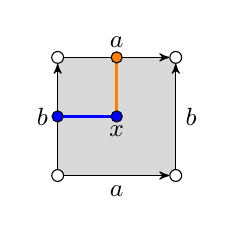
\begin{tikzpicture}[x=1.5cm, y=1.5cm]
      \path[fill=black!15] (0,0) to (1,0) to (1,1) to (0,1);
      \foreach \x in {0, 1} \foreach \y in {0, 1} \node[state] (\x\y)
      at (\x,\y) {};
      \path (00) edge node[below] {$a$} (10);
      \path (01) edge node[above] {$a$} (11);
      \path (00) edge node[left] {$b$} (01);
      \path (10) edge node[right] {$b$} (11);
      \node at (.5,.4) {$\vphantom{b}x$};
    %  \path (00) edge[-, very thick] (01);
   \draw[-, very thick, blue] (0,0.5) -- (.5,0.5);
    \draw[-, very thick, orange] (0.5,0.5) -- (.5,1);
           \node[state, fill=orange, minimum size=0.2mm] at (0.5,1) {};
    \node[state, fill=blue, minimum size=0.2mm] at (0.5,0.5) {};
    \node[state, fill=blue, minimum size=0.2mm] at (0,0.5) {};
    \end{tikzpicture}
    &
    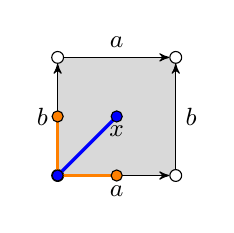
\begin{tikzpicture}[x=1.5cm, y=1.5cm]
      \path[fill=black!15] (0,0) to (1,0) to (1,1) to (0,1);
      \foreach \x in {0, 1} \foreach \y in {0, 1} \node[state] (\x\y)
      at (\x,\y) {};
      \path (00) edge node[below] {$a$} (10);
      \path (01) edge node[above] {$a$} (11);
      \path (00) edge node[left] {$b$} (01);
      \path (10) edge node[right] {$b$} (11);
      \node at (.5,.4) {$\vphantom{b}x$};
     % \node[state, fill=black, minimum size=2mm] at (0,0) {};
      %%%%%%%%%
      \draw[-, very thick, blue] (0,0) -- (.5,0.5);
        \draw[-, very thick, orange] (0,0) -- (.5,0);
           \node[state, fill=orange, minimum size=0.2mm] at (0.5,0) {};
                \draw[-, very thick, orange] (0,0) -- (0,0.5);
           \node[state, fill=orange, minimum size=0.2mm] at (0,0.5) {};
    \node[state, fill=blue, minimum size=0.2mm] at (0.5,0.5) {};
    \node[state, fill=blue, minimum size=0.2mm] at (0,0) {};
    \end{tikzpicture}
    &
   
    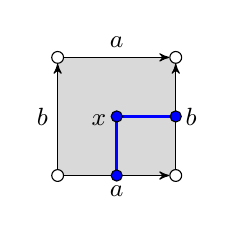
\begin{tikzpicture}[x=1.5cm, y=1.5cm]
      \path[fill=black!15] (0,0) to (1,0) to (1,1) to (0,1);
      \foreach \x in {0, 1} \foreach \y in {0, 1} \node[state] (\x\y)
      at (\x,\y) {};
      \path (00) edge node[below] {$a$} (10);
      \path (01) edge node[above] {$a$} (11);
      \path (00) edge node[left] {$b$} (01);
      \path (10) edge node[right] {$b$} (11);
      \node at (.35,.5) {$\vphantom{b}x$};
   %   \path (00) edge[-, very thick] (10);
   %   \path (10) edge[-, very thick] (11);
%%%%%%%%%%%%
\draw[-, very thick, blue] (0.5,0) -- (.5,0.5) -- (1,0.5);
    \node[state, fill=blue, minimum size=0.2mm] at (0.5,0.5) {};
    \node[state, fill=blue, minimum size=0.2mm] at (0.5,0) {};
\node[state, fill=blue, minimum size=0.2mm] at (1,.5) {};

      
    \end{tikzpicture}
    \\
     $\ev(( \delta_a^0 x \nearrow^a x))= \!\!\ipomset{ & a \ar@{.>}[d]
      \ar[r] & \\ \ar[r] & b \ar[r] &}$ &
    $\ev(( \delta_a^0 \delta_b^0 x \nearrow^{a b } x))= \!\!\ipomset{ & a
      \ar@{.>}[d] \ar[r] & \\ & b \ar[r] &}$ &
   
    $\ev(( \delta_b^0 x \nearrow^b x \searrow_a \delta_a^1 x))= \!\!\ipomset{ \ar[r] & a \ar@{.>}[d]
      \\ & b \ar[r] &}$
  \end{tabular}
  \bigskip
  \caption{Paths and their labels in two-dimensional HDAs }
  \label{fig:label-iface}
\end{figure}
\begin{definition} \label{def: track}
    A precubical map $g: \square^P \to X$ where $P$ is an iipomset is called a track. We say that $g$ is an initial track if $P$ is a discrete pomset and $g(\mathbf{y}_P) = x$ for some $x\in I_X$  .
\end{definition}
\begin{definition}
    Let $X$ be a precubical set. We define the category of tracks $T_X$ as follows
    \begin{itemize}
        \item Objects are tracks $p: \pobj{P} \to X$, where $P$ is an iipomset.
        \item Morhisms are extensions of tracks, that is, $f:p \to p'$ is a morphism of $T_X$ between $p:\pobj{P} \to X$ and $p':\pobj{Q} \to X$ iff $P \ininc Q$. In other words, iff $p'=p \circ \jneda^0_{P\subseteq P*Q}$ .
        \item Composition of $f: [p:\pobj{P} \to X] \to [p':\pobj{P*R} \to X]$ and $g: p' \to [p'':\pobj{P*R*Q} \to X]$ is $g \circ f: p\to p''$.
    \end{itemize}
\end{definition}


%\begin{proposition} \label{prop: generalization of y}
 %   Let $X$ be a precubical set. For all interval pomsets $P$, there exists a unique sparse path $ \rho \in P_{\square^P}$ such that for all $g,g':\square^P \rightarrow X$ if $g(\rho)=g'(\rho)$ then $g=g'$.
    %track $ g: \square^P \rightarrow X$, there exists a unique sparse path $ \rho \in P_{\square^P}$ such that for all $g':\square^P \rightarrow X$ if $g(\rho)=g'(\rho)$ then $g=g'$. \linebreak 
%    In this case, we say that $\rho$ is the characteristic sparse path of $P$.
%\end{proposition}

%\begin{proof}
 %   Let $P=P_1*P_2 \dots * P_{m(P)}$ the sparse decomposition of $P$ into discrete ipomsets.  Induction on $m(P)$:
    %\begin{itemize}
     %   \item  If $P$ is a starter $\subid{U\setminus A}{U}{U}$, then by Yoneda Lemma the unit path $(\mathbf{y}_U)$ meets the requirement.
      %  \item If $P=S*T$ where $S$ is a starter and $T$ is a terminator, then $P$ is a conclist. By yoneda Lemma, $(\mathbf{y}_P)$ meets the requirement.
       % \item If $P=R*Q$ where $m(Q),m(R)<m(P)$, then by Lemma \ref{lemma: pomset pushout} there is a pushout. By induction hypothesis, there exist unique characteristic paths $\rho_0 \in P_{\square^R}$ and $\rho_1 \in P_{\square^Q}$ of $g \circ \jneda^0_{P \subseteq Q}$ and $g \circ \jneda^1$ respectively. Since $\square^P=\jneda^0_{P \subseteq Q}(\square^R)\sqcup \jneda^1(\square^R)$, the path $\jneda^0_{P \subseteq Q}(\rho_0)*\jneda^1(\rho_1)$ meets the requirements.
    %\end{itemize} 
The Yoneda Lemma \ref{lemma: Yoneda lemma} is based on the unique cell $\mathbf{y}_S$ of discrete pomset $S$. For an iipomset $P$, we introduce the characteristic path $\rho_P$ which allows a generalization of the Yoneda lemma by substituting $\rho_P$ for $\mathbf{y}_S$. 
\begin{definition}\label{def: char path}
    Consider $P$ an iipomset. The characteristic path of $P$ is $\rho_P \in P_{\pobj{P}}$ such that $\ev(\rho)=P$, $start(\rho)=I_{\square^P}$, and $end(\rho)=F_{\square^P}$. As a track object is a finite gluing of standard cubes (Theorem \ref{theo: finite gluing of standard cubes}),  $\rho_P$ can be computed by induction
        \begin{itemize}
        \item  If $P$ is a discrete ipomset $\subid{U\setminus A}{U}{U\setminus B}$, then $\rho_P=(\delta^0_A(\mathbf{y}_U),\mathbf{y}_U,\delta^1_B(\mathbf{y}_U))$.
        \item If $P=R*Q$, then $\rho_P=\jneda^0(\rho_R)*\jneda^1(\rho_Q)$, where $\rho_R \in P_{\square^R}$ and $\rho_Q \in P_{\square^Q}$ the characteristic paths of $R$ and $Q$ respectively. 
        
        This is well defined, because $start(\rho_Q)=i_{ \pobj{ Q}}$ and $end(\rho_R)=f_{ \pobj{ R}}$. Denoting by $S \cong T_R \cong S_Q$, we have 
    \begin{equation*}
      start(\rho_Q)(p)=
      \begin{cases}
        \exec & \text{if } p\in S, \\
        0 & \text{if } p\in Q\setminus S,
      \end{cases}
      \qquad
      end(\rho_R)(p)=
      \begin{cases}
        \exec & \text{if } p\in S, \\
        1 & \text{if } p\in R\setminus S;
      \end{cases}
    \end{equation*}
       By Lemma \ref{lemma: pomset pushout}, using the expressions of the initial and final inclusions, we obtain
 \begin{equation*}
      \jneda^1 (start(\rho_Q))(p)=
      \begin{cases}
        \exec & \text{if } p\in S, \\
        1 & \text{if } p\in R \setminus S, \\
        0 & \text{if } p\in Q\setminus S,
      \end{cases}
     =\jneda^0 (end(\rho_R))(p)
    \end{equation*}
     Thus, the paths $\jneda^0(\rho_R)$ and $\jneda^1(\rho_Q)$ can be concatenated in $\square^P$. %It is easy to check that the path  meets the requirements.
    \end{itemize} 
\end{definition}
\begin{remark}
    As a result of our construction of the characteristic path, we get a sparse path. It is possible, however, for the same construction to result in a path that is not sparse. All paths resulting from this construction are congruent overall. Thus, the sparse path is unique up to the congruence relation.
\end{remark}


 %   \begin{proof}
  %       Let $P=P_1*P_2 \dots * P_{m(P)}$ be the minimal discrete decomposition of $P$ into discrete ipomsets. We employ an induction on $m(P)$.    
  %  \end{proof}
The following proposition generalizes Yoneda Lemma \ref{lemma: Yoneda lemma}. Instead of cells, here we have paths, and instead of conclists, we have iipomsets. 
\begin{proposition} \label{prop: prop: generalization of yoneda }
    Let X be a precubical set, P an iipomset, $ \alpha \in \mathrm{P}_{X}$, and $\rho_P$ the characteristic path of $P$.
    If $\ev (\alpha)=P$, then there exists a unique track $g_{\alpha} :\square^P \rightarrow X$ such that $g_{\alpha} (\rho_P)=\alpha$.
\end{proposition}
\begin{proof}

Induction on the number of cells of $\alpha$.
    \begin{itemize}
        \item If $\alpha=(x)$ then $P=\ev (x)$. The path $\alpha'=(\mathbf{y}_P)$ and the Yoneda embedding $\iota_{x}$ satisfy the requirement. 
        \item If $\alpha=(y\nearrow^A x)$, then $P= \subid{\ev(x) \setminus A}{\ev(x)}{\ev(x)} $. We may take $g_{\alpha}=\iota_x$ and \linebreak $\alpha'=(\delta^0_A(\mathbf{y}_U),\mathbf{y}_U)$, where $U=\ev(x)$.  
         \item If $\alpha=(x\searrow^B y)$, then $P= \subid{\ev(x)}{\ev(x)}{\ev(y)\setminus B} $. Again, we may take $g_{\alpha}=\iota_x$ and $\alpha'=(\mathbf{y}_U,\delta^1_A(\mathbf{y}_U))$, where $U=\ev(x)$.  
        \item If $\alpha=\beta*\theta$ where both $\beta$ and $\theta$ are shorter than $\alpha$. Let $R=\ev(\beta)$ and $Q=\ev(\theta)$ (we therefore have $P=R*Q$). By induction hypothesis, there exist a unique $g_{\beta}:\square^R \rightarrow X$, and a unique $g_{\theta}:\square^Q \rightarrow X$, such that $g_{\beta}(\rho_R)=\beta$ and $g_{\theta}(\rho_Q)=\theta$. %$g_{\beta}(i_{\square^R})=start(\beta)$, $g_{\theta}(f_{\square^Q})=end(\theta)$, and $g_{\theta}(i_{\square^R})=g_{\beta}(f_{\square^R})$. 
         By Lemma \ref{lemma: pomset pushout}, $g_{\theta}$ and $g_{\beta}$ glue to a map $g_{\alpha}: \square^P \rightarrow X$, which satisfies the requirements.
        %The $\rho=(\xi)$, where $\xi$ is the unique cell of dimension $\midP\mid$, and the yoneda embedding $\iota_{x}$ satisfy the requirement. 
    \end{itemize}
\end{proof}
There is a shared unique track of the previous proposition for congruent paths. In other words, if $\alpha \simeq \beta$ then $g_{\alpha}=g_{\beta}$. The next theorem gives more details on this.
\begin{theorem}\label{th: path and tracks isomorphism}
    Let $X$ be a precubical set. The categories $\mathbb{P}_{X}$ and $T_X$ are isomorphic.
\end{theorem}
\begin{proof}
     The following map is a functor.
    \begin{align*}
        \psi: \mathbb{P}_{X} & \to  T_X \\
        \text{for } \alpha \in Obj(\mathrm{P}_{X}), & ~ \psi(\alpha)= g_{\alpha} \\
        \text{for } f:\alpha \to \alpha*\beta, &~ \psi(f): g_{\alpha}\to g_{\alpha*\beta}.
    \end{align*}
    Note that $f$ induces an iipomset map $f: \ev(\alpha) \to \ev(\alpha)*\ev(\beta) $ such that $\square^f$ is the initial inclusion $\jneda^0_{\ev(\alpha)\subseteq \ev(\alpha)*\ev(\beta)}$ and $g_{\alpha}= g_{\alpha*\beta} \circ \square^{f}$ so we obtain
    
    $$\psi(f): [g_{\alpha*\beta} \circ \square^{f} : \pobj{\ev(\alpha)} \to X] \to [g_{\alpha*\beta}: \pobj{\ev(\alpha)*\ev(\beta)} \to X].$$

    The inverse of $\psi$ is given  by
     \begin{align*}
        \varphi: T_X & \to  \mathbb{P}_{X} \\
        \text{for } p: \pobj{P}\to X \in Obj(T_X), & ~ \varphi(p)= p(\rho_P) \\
        \text{for } f: [p: \pobj{P} \to X] \to [p: \pobj{P*R} \to X], &~ \varphi(f): p(\rho_P) \to p(\rho_P)*p'\circ \jneda^1_{R\subseteq P*R}(\rho_R)
    \end{align*}

    We remind the reader that $\rho_{P*R}=\jneda^0_{P\subseteq P*R} (\rho_P)* \jneda^1_{R\subseteq P*R}(\rho_R)$ and that $ p'\circ \jneda^0_{P\subseteq P*R}=p$, thus $\varphi(f)(p)=p'(\rho_{P*R})$. To show that $\varphi$ is a functor, let $f:p\to p'$ and $g:p'\to p''$. On one hand, we have \linebreak $\varphi(g \circ f)(p)= p(\rho_P)*p''\circ \jneda^1_{R*Q\subseteq P*R*Q}(\rho_{R*Q})=p(\rho_P)*p''\circ \jneda^1_{R*Q\subseteq P*R*Q}(\jneda^0_{R\subseteq R*Q} (\rho_R)* \jneda^1_{Q\subseteq R*Q}(\rho_Q))$. On the other hand, we have $p(\rho_P) \stackrel{\varphi(f)}{\longrightarrow} p'(\rho_{P*R})\stackrel{\varphi(g)}{\longrightarrow} p''(\rho_{P*R*Q})$, so $\bigl(\varphi(g)\circ \varphi(f)\bigl)(p)=p'(\rho_{P*R})*p''\circ \jneda^1_{Q\subseteq P*R*Q}(\rho_Q)=(p(\rho_{P})*p'\circ \jneda^1_{R\subseteq P*R}(\rho_R))*p''\circ \jneda^1_{Q\subseteq P*R*Q}(\rho_Q)$. To show that $\varphi(g \circ f)(p)=\bigl(\varphi(g)\circ \varphi(f)\bigl)(p)$, it is enough to show that 
    \begin{equation}\label{eq: in the proof}
        p''\circ \jneda^1_{R*Q \subseteq P*R*Q} \circ \jneda^0_{R\subseteq R*Q}=p'\circ \jneda^1_{R\subseteq P*R}
    \end{equation}
    Using the expression of initial and final inclusions (Lemma \ref{lemma: pomset pushout}), an elementary calculation shows that $\jneda^1_{R*Q \subseteq P*R*Q} \circ \jneda^0_{R\subseteq R*Q}=\jneda^0_{P*R\subseteq P*R*Q}\circ \jneda^1_{R\subseteq P*R}$, meaning that the square in the followig diagram commutes. Thus, $ p''\circ \jneda^1_{R*Q \subseteq P*R*Q} \circ \jneda^0_{R\subseteq R*Q}= p''\circ \jneda^0_{P*R\subseteq P*R*Q}\circ \jneda^1_{R\subseteq P*R}$ and (\ref{eq: in the proof}) follows since $p''\circ \jneda^0_{P*R \subseteq P*R*Q} =p'$

 $$\xymatrix{
    & \pobj{R} \ar[r]^{\jneda^0} \ar[d]^{\jneda^1}&  {\pobj{R*Q}} \ar[d]^{\jneda^1}  \\ \pobj{P} \ar[dr]_{p} \ar[r]^{\jneda^0} &  {\pobj{P*R}} \ar[r]^{\jneda^0} \ar[d]_{p'} &  \pobj{P*R*Q}  \ar[dl]^{p''}  \\   & X &    }
$$

The equalities $\psi \circ \varphi = \mathbf{id}_{T_X}$ and $ \varphi \circ \psi = \mathbf{id}_{\mathbb{P}_{X}}$ can be checked using the definition \ref{def: char path} of the characteristic path and Proposition \ref{prop: prop: generalization of yoneda }. 
  
\end{proof}

    %%%%%%%%%%%%%%%%%%%%%%%%%%%%%
%$g=g' \forall i$. Therefore, $g=g'$. 
%Assume that $\rho=(\xi_1, \xi_2, \dots, \xi_s)$ satisfies the requirement. 
%Now, if $P=R*P_{s+1}$, let  $g': \square^P \rightarrow X$ such that $g'(\rho*(\xi_{s+1})))=g(\rho*(\xi_{s+1})))$. By proposition \ref{prop: map characterizations}, there exists an initial inclusion $\jneda^0_{P \subseteq Q} :\square^R  \rightarrow \square^P$ and a final inclusion $J_1 :\square^{P_{s+1}}  \rightarrow \square^P$. By induction hypothesis, $g \circ \jneda^0_{P \subseteq Q} =g' \circ \jneda^0_{P \subseteq Q}$  and again by Yoneda Lemma $g \circ J_1 =g' \circ J_1$. Since $\square^P=\jneda^0_{P \subseteq Q}(\square^R)\cup J_1(\square^R)$ (as there is a pushout by Lemma 65 \cite{LanguageofHDA}), thus $g=g'$.

%\begin{remark}
 %      Let $P$ and $R$ be composable iipomset and $Q=P*Q$. By Lemma \ref{lemma: pomset pushout}, there is a pushout.
       
  %     the initial and final inclusion $J^0$ and $J^1$ respectively. Then the characteristic path 
%\end{remark}
\section{Bisimulation and modal logic}\label{Sec: bis and ml}
\subsection{Overwiew for bisimulation from open maps}\label{subsec: open map}
\begin{description}
    \item[\hspace{0.5cm} Path lifting property]
  Let $\mathbf{C}$ be a subcategory of $\widehat{\square}$ and $X,Y$ precubical sets. A precubical map $\varphi: X \to Y$ has the path lifting-property with respect to $\mathbf{C}$ if whenever for $v \in \hom_{\mathbf{C}}: P \to Q$, $p: P \rightarrow X$ and $q: Q \rightarrow Y$, $q \circ v = \varphi \circ p$ i.e the following diagram $$
% \begin{equation*}
    \xymatrix{%
      P \ar[r]^{p}
      \ar[d]_{v} \ar@{}[dr]  &
      X \ar[d]^{\varphi} \\
      Q \ar[r]_{q}  & Y 
    }
 % \end{equation*}
$$
commutes, %meaning that the track $\varphi \circ p$ can be extended into a track q via m, 
then there exists a morphism $p'$ such that $p'\circ v=p$ and $\varphi \circ p'=q$ i.e the two triangles in the following diagram commute

$$
% \begin{equation*}
    \xymatrix{%
      P \ar[r]^{p}
      \ar[d]_{v} \ar@{}[dr]  &
      X \ar[d]^{\varphi} \\
      Q  \ar[r]_{q} \ar[ur]_{p'} & Y  
    }
 % \end{equation*}
$$
 In this case, we say that $\varphi$ is $\mathbf{C}$-open or that $\varphi$ is open with respect to $\mathbf{C}$. Similarly, an HDA map $\varphi: \mathcal{X} \to \mathcal{Y}$ is said to be open with respect to $\mathbf{C}$, if $\varphi$ satisfies the path-lifting property. This gives rise to a notion of bisimulation with respect to $\mathbf{C}$. 
 \begin{definition} \label{def: U bis from open map}
Let $\mathcal{Y}$, $\mathcal{Z}$ be HDAs. We say that $\mathcal{Y}$ and $\mathcal{Z}$ are $\mathbf{C}$-bisimilar if there is a span of $\mathbf{C}$-open HDA maps $\mathcal{Y} \stackrel{\varphi}{\longleftarrow} \mathcal{X} \stackrel{\psi}{\longrightarrow} \mathcal{Z}$ with a common HDA $\mathcal{X}$.
     \end{definition} 

\item[\hspace{0.5cm} The future lifting property]  A precubical map $\varphi: X \to Y$ has the future lifting property (FLP) if for every up-step $\beta=(\varphi(x) \nearrow^A y)$ in $Y$, there exists an up-step $\alpha=(x \nearrow^A x')$ in $X$ such that $\varphi(\alpha)=\beta$. 
%\item[\hspace{0.5cm} The past lifting property]  A precubical map $\varphi: X \to Y$ has past lifting property (PLP) if for every down-step $\beta=(\varphi(x) \searrow_A y)$ in $Y$, there exists down-step $\alpha=(x \searrow_A x')$ in $X$ such that $\varphi(\alpha)=\beta$.

\item[\hspace{0.5cm} The the future path lifting property]  A precubical map $\varphi: X \to Y$ has the the future path lifting property if for $\alpha \in \mathrm{P}_{X}$ and $\beta \in P_Y$, if $\varphi(\alpha) \text{ and } \beta$ can be concatenated, then there exists $\alpha'$ in $X$ such that $\alpha \text{ and } \alpha^{\prime}$ can be concatenated and $\varphi(\alpha * \alpha^{\prime})=\varphi(\alpha)* \beta$.
\end{description}


\subsection{Characterization of bisimulation from $\TrO^0$-open map}
In this section, we will apply the previous general approach, focusing on $\TrO^0$ as subcategory of $\widehat{\square}$.
\begin{lemma} \label{Lemma: Zig Zag property for U}
For any precubical map $\varphi: Y \rightarrow X$ the following conditions are equivalent:
\begin{enumerate}
    \item $\varphi$ is $\TrO^0$-open;
    \item $\varphi$ has the FLP;
    \item $\varphi$ has the future path lifting property.
    
\end{enumerate}
\end{lemma}
\begin{proof}
$1 \Rightarrow 2$ Let $x\in X$ and $\alpha=(\varphi(x)\nearrow^A y)$, $\ev (\alpha)=U$, and $d^0_A$ be the face map that corresponds to the initial inclusion $(f_A,\varepsilon_0): U\setminus A \to U$. As $\varphi(x)=\delta_A^0(y)$, 
\begin{align} \label{eq: from yoneda of f(x)}
\varphi \circ \iota_{x}(\mathbf{y}_{U\setminus A})=\delta_A^0(y)    
\end{align}
On the other hand, by elementary calculation, $\delta_A^0(\mathbf{y}_U)=\square^{d_A^0}(\mathbf{y}_{U\setminus A})$. Thus, 
\begin{align*}
\iota_{y}(\delta_A^0(\mathbf{y}_U)) & =\iota_{y} (\square^{d_A^0}(\mathbf{y}_{U\setminus A}))\\
& = \delta_A^0(\iota_{y}(\mathbf{y}_U)) \text{ as the face maps commute with the natural tranformation } \iota_y\\
& = \delta_A^0(y) \\
& \stackrel{(\ref{eq: from yoneda of f(x)})}{=} \varphi \circ \iota_{x}(\mathbf{y}_{U\setminus A}) 
\end{align*}
Thus $\iota_{y} \circ \square^{d_A^0}(\mathbf{y}_{U\setminus A})=\varphi \circ \iota_{x}(\mathbf{y}_{U\setminus A})$. By Yoneda Lemma, $\iota_{y} \circ \square^{d_A^0}=\varphi \circ \iota_{x}$, meaning that the following diagram commutes.
$$    \xymatrix{%
      \square^{U\setminus A} \ar[r]^{\iota_{x}}
      \ar[d]_{\square^{d_A^0}} \ar@{}[dr]  &
      X \ar[d]^{\varphi} \\
      \square^U  \ar[r]_{\iota_{y}} \ar@{.>}[ur]_{\iota_{x'}}  & Y  
    }
$$
Since $\varphi$ is $\TrO^0$-open, there exists $\iota_{x'}: \square^{U} \to Y$ such that $\iota_{x'} \circ \square^{d_A^0}= \iota_{x}$ and $ \varphi \circ \iota_{x'} = \iota_{y}$. Thus, %$ \varphi \circ \iota_{x'} (\mathbf{y}_U) = \iota_{y} (\mathbf{y}_U)=y$ and $\iota_{x'} \circ \square^{d_A^0}(\mathbf{y}_{U\setminus A})=\iota_{x'}  \bigl(\delta_A^0(\mathbf{y}_{U})\bigl)=\delta_0^A  \bigl(\iota_{x'}(\mathbf{y}_{U})\bigl)= \iota_{y}(\mathbf{y}_{U\setminus A})=y$. That is 
for $x'=\iota_{x'}(\mathbf{y}_{U})$, we have $\beta=(x \nearrow^Ax')$ in $Y$ and $\varphi(\alpha)= \beta$. The PLP follows in a similar way.

$2 \Rightarrow 3$ and $3 \Rightarrow 2$ are immediate.

$3\Rightarrow 1$ Let $\varphi: X \rightarrow Y$ be a map, $\jneda^0_{P \subseteq Q} : \square^P \rightarrow \square^Q$ an initial inclusion, and $q: \square^Q \rightarrow Y$ such that
\begin{equation} \label{eq: hyp from open map}
 \varphi \circ p = q \circ \jneda^0_{P \subseteq Q}   
\end{equation}
Let $\rho_P$ and $\rho_Q$ be the characteristic paths of $P$ and $Q$ respectively. By Definition \ref{def: char path}, we have $\rho_Q= \jneda^0_{P \subseteq Q}(\rho_P)* \sigma$ for some $\sigma \in P_{\pobj{Q}}$, hence 
$q(\rho_Q)=q\circ \jneda^0_{P \subseteq Q} (\rho_P)* q(\sigma)$. Defining $\alpha=p(\rho_P)$ and $\beta=q(\sigma)$, we obtain by (\ref{eq: hyp from open map}), $q(\rho_Q)=\varphi(\alpha)* \beta$. The future path lifting property yields a path $\alpha'$ such that $\varphi(\alpha*\alpha')=\varphi(\alpha)*\beta$. Since $\ev(\alpha*\alpha')= \ev(q(\rho_Q))=Q$, by Proposition \ref{prop: prop: generalization of yoneda }, there exists a unique track %$g_{\alpha'}: \pobj{R} \to X$ such that 
$g: \pobj{Q} \to X$ such that $g(\rho_Q)=\alpha*\alpha'$. On one hand $g \circ \jneda^0_{P \subseteq Q} (\rho_P)= \alpha = p(\rho_P)$, %just not so sure why g \circ \jneda^0_{P \subseteq Q} (\rho_P)= \alpha (well if we define g in two steps and then take as the gluing, it will be fine).
thus by Proposition \ref{prop: prop: generalization of yoneda }, $g \circ \jneda^0_{P \subseteq Q} = p$. On the other hand, 
$\varphi \circ g (\rho_Q)= \varphi (\alpha*\alpha') = q (\rho_Q)$ thus again by Proposition \ref{prop: prop: generalization of yoneda } $\varphi \circ g = q$. Therefore, $\varphi$ is $\TrO^0$-open.  
%The idea of the proof is to rely on Definition \ref{def: char path} to find paths $\alpha \in P_Y$ and $\beta \in \mathrm{P}_{X}$, such that $\varphi(\alpha)$ and $\beta$ can be concatenated. The the future path lifting property yields a path $\alpha'$ such that $\varphi(\alpha*\alpha')=\varphi(\alpha)*\beta$. We use Proposition \ref{prop: prop: generalization of yoneda } to construct a track that meets the requirement of the path lifting property.
\end{proof}

%\begin{remark}
%    \textcolor{red}{If we consider only inital paths (every path starts from an initial cell), then  all $\mathcal{U}$- bisimulations are maximal.} This can be shown by induction on the length of the path. Otherwise we will get the following spectrum 
  %  If we add the following weeker condition: for all $x\in X$ there exists an initial cell $i$ and a path $\alpha: i \leadsto x$, then our bisimulation should respect the second part of the restriction: meaning that "for all $( \rho, \sigma)\in R$ and paths $\rho'$ on $Y$ and $\sigma'$ in $Z$ of the same length such that $\rho=\rho'*\rho''$ and $\sigma=\sigma'*\sigma''$ for some $\rho''$ and $\sigma''$, $( \rho'',\sigma'')\in R$;"
%\end{remark} 

\begin{definition}\label{def: U bar bis}
     A \emph{$\overline{\mathcal{U}}$-bisimulation} between HDAs $\mathcal{Y}$ and $\mathcal{Z}$ is a relation $\overline{R}$ between cells in $Y$ and $Z$ such that
\begin{enumerate}
\item \label{en: U bar bisim.e1} for any $ y\in I_Y $, $\emptyset \neq \{z \in Z \mid (y,z) \in R \} \subseteq I_Z$ and vice versa;
%there exists $ z \in I_Z$ such that $(y,z)\in R$ and vice versa. In addition, if $x \in Z$ such that $(y,z)$
%\item \label{en: U bisim.e2} $R$ respects final cells: for all
\item \label{en: U bar bisim.e3} $\overline{R}$ respects labels: for all
  $( y, z)\in \overline{R}$, $\ev_Y( x)= \ev_Z(y)$;
\item \label{en: U bar bisim.e4} for all $( y, z)\in \overline{R}$, for all $A \subseteq \ev_Y(x)= \ev_Z(y)$, $( \delta^{\nu}_A(y),
 \delta^{\nu}_A(z))\in \overline{R}$; %The case where \nu=1 concerns the extension (in case of terminating an event) of for both ways (from Y to Z and vice versa). The case where \nu=0 concerns the faces preservation.
\item \label{en: U bar bisim.e5} for all $( y, z)\in \overline{R}$, if there exists $y'$ such that $\delta^{0}_A(y')=y$ for some $A\subseteq \ev(y')$, then there exists $z'$ such that $\delta^{0}_A(z')=z$ and $( y', z') \in \overline{R}$; %this concerns the restrictions of for both ways (from Y to Z and vice versa)

\item \label{en: U bar bisim.e6} for all $( y, z)\in \overline{R}$, if there exists $z'$ such that $\delta^{0}_A(z')=z$ for some $A\subseteq \ev(z')$, then there exists $y'$ such that $\delta^{0}_A(y')=y$ and $( y', z') \in \overline{R}$; %this concerns the restrictions for both ways (from Y to Z and vice versa)
%\item \label{en: U bar bis initial faces preservation} 
\end{enumerate}
\end{definition}
%%%%%%%%%%%%%%%%%%%%%On a cette implication autrement.
%\begin{proposition}\label{prop: U bar implies U}
 %   If two HDAs $\mathcal{Y}$ and $\mathcal{Z}$ are \emph{$\TrO^0$-bisimilar} then they are \emph{$\mathcal{U}$-bisimilar}. 
%\end{proposition}
%\begin{proof}
 %Assume that there is a span of $\TrO^0$-open maps $\mathcal{Y} \stackrel{\varphi}{\longleftarrow} \mathcal{X} \stackrel{\psi}{\longrightarrow} \mathcal{Z}$. We show that the relation $K=\{ (\varphi(\alpha), \psi(\alpha)) , \alpha \in \mathrm{P}_{X} \}$ is a $\mathcal{U}$-bisimulation. The first property is satisfied since $\varphi$ and $\psi$ preserve initial cells. By \cite[Lemma 27]{LanguageofHDA}, $K$ respects labels. To show \ref{en: U bisim.e4}, we consider two related paths $(\varphi(\alpha),\psi(\alpha))$ for some $\alpha \in \mathrm{P}_{X}$. Assume that $\varphi(\alpha)$ can be concatenated with some $\beta \in P_Y$. By Lemma \ref{Lemma: Zig Zag property for U}, there exists $\alpha' \in \mathrm{P}_{X}$ such that $\alpha$ and $\alpha'$ can be concatenated and $\varphi(\alpha*\alpha')=\varphi(\alpha)*\beta$. As $\psi(\alpha)$ and $\psi(\alpha')$ can be concatenated, $(\varphi(\alpha)*\beta, \psi(\alpha)*\psi(\alpha'))=(\varphi(\alpha*\alpha'), \psi(\alpha*\alpha')) \in K$. We can show that $K$ satisfies \ref{en: U bisim.e5} similarly.
%\end{proof}
%\end{definition}
\begin{theorem} \label{U and T bis}
Two HDAs $\mathcal{Y}$ and $\mathcal{Z}$
    %\item If $\mathcal{Y}$ and $\mathcal{Y}$ are $\TrO^0$-bisimilar then they are % this is correct but can be deducted from the previous proposition 
    are $\TrO^0$-bisimilar iff they are \emph{$\overline{\mathcal{U}}$-bisimilar}.  
\end{theorem}

\begin{proof}
    $"\Rightarrow"$ Assume that there is a span of HDA $\TrO^0$-open maps $\mathcal{Y} \stackrel{\varphi}{\longleftarrow} \mathcal{X} \stackrel{\psi}{\longrightarrow} \mathcal{Z}$. 
    The relation $K=\{ (\varphi(x), \psi(x)) , x \in X \}$ is a $\overline{\mathcal{U}}$-bisimulation. Let $y \in I_Y$, since $\varphi(I_X)=I_Y$, there exists $x\in I_X$ such that $\varphi(x)=y$. Again as $\psi$ is an HDA map, $\psi(x)\in I_Z$, thus \ref{def: U bar bis}. \ref{en: U bar bisim.e1} is satisfied. By \cite[Lemma 27]{LanguageofHDA}, $K$ respects labels, thus \ref{def: U bar bis}.\ref{en: U bar bisim.e3} is satisfied. 
    Condition \ref{def: U bar bis}.\ref{en: U bar bisim.e4} is satisfied as $\varphi$ is a precubical map. To show \ref{def: U bar bis}.\ref{en: U bar bisim.e5} and similarly \ref{def: U bar bis}.\ref{en: U bar bisim.e6}, let  $(y,z)=(\varphi(x),\psi(x))$. Assume that there exists $y' \in Y$ such that $\delta_A^0(y')=y$. Since $\varphi$ is open, by Lemma \ref{Lemma: Zig Zag property for U}, there exists an up step $\alpha=(x \nearrow^A x')$ in $ X$ such that $\varphi(\alpha)=(y \nearrow^A y')$. Defining $z'=\psi(x')$ we obtain $\delta_A^0(z')=z$ and $(y',z') \in K$.
     %To show \ref{en: U bisim.e4}, we consider two related paths $(\varphi(\alpha),\psi(\alpha))$ for some $\alpha \in \mathrm{P}_{X}$. Assume that $\varphi(\alpha)$ can be concatenated with some $\beta \in P_Y$. By Lemma \ref{Lemma: Zig Zag property for U}, there exists $\alpha' \in \mathrm{P}_{X}$ such that $\alpha$ and $\alpha'$ can be concatenated and $\varphi(\alpha*\alpha')=\varphi(\alpha)*\beta$. As $\psi(\alpha)$ and $\psi(\alpha')$ can be concatenated, $(\varphi(\alpha)*\beta, \psi(\alpha)*\psi(\alpha'))=(\varphi(\alpha*\alpha'), \psi(\alpha*\alpha')) \in K$. We can show that $K$ satisfies \ref{en: U bisim.e5} similarly. Finally, $K$ satisfies \ref{en: U bisim.e6} because the restrictions of $\varphi(\alpha)$ and $\psi(\alpha)$, of length $m$, are, respectively, $\varphi(\alpha')$ and $\psi(\alpha')$ where $\alpha'$ is a restriction of $\alpha$ of length $m$. 

    
        $"\Leftarrow"$ Assume that there exists a $\overline{\mathcal{U}}$-bisimulation $R$ between $\mathcal{Y}$ and $\mathcal{Z}$. Let $\mathcal{X}=(X,(I_Y \times I_Z)\cap R, F_Y \times F_Z)$ where $X=R$ and $\delta_A^{\nu}(y,z)=(\delta_A^{\nu}(y),\delta_A^{\nu}(z))$. Let $\varphi$ and $\psi$ be projections which for $(y,z) \in X$ give $y$ and $z$ respectively. By condition \ref{def: U bar bis}.\ref{en: U bar bisim.e1}, $\varphi$ and $\psi$ preserve initial cells.  Let $(y,z)\in X$, and then an up-step $\beta=\bigl(\varphi(y,z) \nearrow^A y'\bigl)$ in $Y$. %Defining $\rho \in P_Y$ and $\sigma \in P_Z$ such that $(start(\rho),start(\sigma)) \in I_Y \times I_Z$, $end(\rho)=y$, and $end(\sigma)=z$ we obtain 
        As $(y,z) \in R$, by \ref{def: U bar bis} .\ref{en: U bar bisim.e5}, there exists $z' \in Z$ such that $z \nearrow^A z'$ and $(y',z') \in R$. That is, there exists an up-step $\alpha=((y,z) \nearrow^A (y',z'))$ in $X$ such that $\varphi(\alpha)=\beta$. Thus, $\varphi$ satisfies the FLP. By Lemma \ref{Lemma: Zig Zag property for U}, $\varphi$ is $\TrO^0$-open. We can show that $\psi$ is $\TrO^0$-open in a similar way.
        \end{proof}
%The condition strong makes the correspendant cells of the related path related by the relation U bar. In terms of the definition of X, I think that it makes the defintiion of X as a non-dijoint union. If U was not a strong U bisimulation, what would happen? Another question, that I still don't know its answer: Is X really an HDA? still lack examples and intuitions
\subsection{Modal characterization}
We introduce a Hennessy-Milner logic and show that it is characteristic to $\mathcal{U}$-bisimulation.

        \begin{definition}\label{def: track bisimulation}
     A track bisimulation, with respect to $\TrO^0$, between HDAs $\mathcal{Y}$ and $\mathcal{Z}$ is a set $R$ of pairs of tracks $\left(p_{1}, p_{2}\right)$ with common domain $\square^P$, so $p_{1}: \square^P \rightarrow Y$ is a track in $Y$ and $p_{2}: \square^P \rightarrow Z$ is a track in $Z$, such that
\begin{enumerate}
    \item \label{eq1: track bis} all initial track in $Y$ are related to an initial track in $Z$ and vice-versa;
    %Initial tracks are related: The set $\{ \}$ letting $p_{1}, p_{2}$ be the unique tracks $p_{1}: y_0 \rightarrow X_{1}$ and $p_{2}: z_0 \rightarrow X_{2}$ from the initial object, $\left(p_{1}, p_{2}\right) \in R$.
    \item \label{eq2: track bis} For $\left(p_{1}, p_{2}\right) \in R$, if $p_{1}^{\prime} \circ \jneda^0_{P \subseteq Q}=p_{1}$, with $\jneda^0_{P \subseteq Q}$ is a morphism of $\TrO^0$, in the following diagram
$$\xymatrix{
     &    \square^P \ar[dl]_{p_1} \ar[d]_{\jneda^0_{P \subseteq Q}} \ar[dr]^{p_2}   \\
   Y & \square^Q \ar[l]^{p'_1 } \ar@{.>}[r]_{p'_2} &  Z                          }
$$
then there is $p'_2$ such that $(p'_1,p'_2) \in R$ and $p'_2 \circ\jneda^0_{P \subseteq Q}=p_2$. %\ar@{.>}[r]
We say a track bisimulation is strong if, in addition, it satisfies:
\item \label{eq3: track bis}  If $(p_1,p_2) \in R$ with $p_{1}: \square^Q \rightarrow Y$ and $p_{2}: \square^Q \rightarrow Z$ and $\jneda^0_{P \subseteq Q}: \square^P \rightarrow \square^Q$, as showed in the following diagram,

$$\xymatrix{
     &    \square^P  \ar[d]_{\jneda^0_{P \subseteq Q}}  \\
   Y & \square^Q \ar[l]^{p_1 } \ar[r]_{p_2} &  Z                          }
$$

then $(p'_1,p'_2)=(p_1 \circ \jneda^0_{P \subseteq Q},p_2 \circ \jneda^0_{P \subseteq Q}) \in R$.

$$\xymatrix{
     &    \square^P \ar[dl]_{p'_1} \ar[d]_{\jneda^0_{P \subseteq Q}} \ar[dr]^{p'_2}   \\
   Y & \square^Q \ar[l]^{p_1 } \ar[r]_{p_2} &  Z                          }
$$

We say that two HDAs are (strong) track bisimilar iff there is a (strong) track bisimulation between them.
\end{enumerate}
\end{definition}

Path assertions are given by
$$
F,G::= \top \mid \bot \mid F \wedge G \mid F \vee G  \mid\langle \jneda^0_{P \subseteq Q} \rangle F\mid  \overline{\langle \jneda^0_{P \subseteq Q}\rangle} F,
$$

Where $\jneda^0_{P \subseteq Q}$ is a morphism in $\TrO^0$. The modality $\overline{\langle \jneda^0_{P \subseteq Q}\rangle}$ is a backward modality, while $\langle \jneda^0_{P \subseteq Q}\rangle$ is a forward modality. 

 The satisfaction relation between a track $p: \square^P \rightarrow X$ and a formula $F$ is given by structural induction on assertions as follows:
 \begin{itemize}
\item $p \models \top$ for all $p$. 
\item $p \models \bot$ for no $p$. 
\item $p \models F \wedge G$ iff $p \models F $ and $p \models G$,
\item $p \models F \vee G$ iff $p \models F $ or $p \models G$,
\item $p \models \overline{\langle \jneda^{0}\rangle} F$ with $\jneda^{0}: \square^Q \rightarrow \square^{P} $, iff  $q \models F$ where $q= p \circ \jneda^{0} : \square^{Q}  \rightarrow X$
\item $p \models \langle \jneda^0_{P \subseteq Q} \rangle F$ with $\jneda^0_{P \subseteq Q}: \square^{P} \rightarrow \square^Q$, iff there is a track $q: \square^Q  \rightarrow X$ for which $q \models F$ and $p=q \circ \jneda^0_{P \subseteq Q}$.
\end{itemize}
By theorem \ref{th: path and tracks isomorphism}, the previous modal logic, given with satisfaction relation on tracks, induces a modal logic interpreted over paths, where congruent paths satisfy the same formulas. The induced satisfaction relation is thus a binary relation $\models$ that relates $\alpha \in \mathrm{P}_X$ to formulae, given by structural induction as follows: 
 \begin{itemize}
\item $\alpha \models \top$ for all $\alpha$. 
\item $\alpha \models \bot$ for no $\alpha$. 
\item $\alpha \models F \wedge G$ iff $\alpha \models F $ and $\alpha \models G$,
\item $\alpha \models F \vee G$ iff $\alpha \models F $ or $\alpha \models G$,
\item $\alpha \models \overline{\langle R \rangle} F$ with $R$ an iipomset, iff  $\alpha' \models F$ where $\alpha= \alpha'*\beta$ and $\ev(\beta)=R$.
\item $\alpha \models \langle R \rangle F$ with $R$ an iipomset, iff there is $\beta \in P_X$ for which $\alpha*\beta \models F$ and $\ev(\beta)=R$.
\end{itemize}

\begin{example}
   As shown in Fig. \ref{fig:label-iface}, let $\alpha_1$ be the path on the left and $\alpha_2$ be the path in the middle, and $\alpha_3$ be the path on the right, we have:
\begin{itemize}
    \item $\alpha_1 \models  \langle  R \rangle \top$, where $R=\!\!\ipomset{ \ar[r] & a \ar@{.>}[d]
     & \\ \ar[r] & b \ar[r] &}$, thus $\beta= (x,\delta^1_a x)$. Note that $R$ is a terminator of the event $a$, thus the formula indicates that there is an extension of $\alpha$ that terminates $a$.  The case of a starter can be interpreted similarly.
     \item $\alpha_2 \models \overline{ \langle  R \rangle} \top$, where $R=\!\!\ipomset{ \ar[r] & a \ar@{.>}[d]  \ar[r]
     & \\  & b \ar[r] &}$ thus $\alpha'= (\delta_a^0 \delta_b^0 x \nearrow^{a } \delta_b^0 x)$. Note that $R$ is a starter of the event $b$, thus the formula indicates that there is a restriction of $\alpha$ that unstarts $b$.  The case of a terminator can be interpreted similarly.
     \item $\alpha_2 \nvDash  \langle  R \rangle \top$, where $R=\!\!\ipomset{  & c \ar@{.>}[d]  \ar[r]
     & \\ \ar[r] & d \ar[r] &}$. Intuitively, the formulae indicated that there is no 2-dimensional $y$ with $\ev(y)=\!\!\ipomset{ \ar[r] & c \ar@{.>}[d]  \ar[r]
     & \\ \ar[r] & d \ar[r] &}$ that can be glued to the cell $x$.
     
\end{itemize}

\end{example}

\begin{theorem} \cite{JOYAL1996164}
Let $\mathcal{Y}$ and $\mathcal{Z}$ two HDAs.
    \begin{itemize}
        \item $\mathcal{Y}$ and $\mathcal{Z}$ are track bisimilar iff initial tracks satisfy the same forward-track assertions. 
        \item $\mathcal{Y}$ and $\mathcal{Z}$ are strong track bisimilar iff initial tracks satisfy the same path assertions.
    \end{itemize}
\end{theorem}

%\begin{proof}
%    $"\Rightarrow"$ Assume $R$ is a track bisimulation between HDAs $\mathcal{Y}$ and $\mathcal{Z}$.
%\end{proof}

\begin{theorem}
   If two HDAs $\mathcal{Y}$ and $\mathcal{Z}$ are $\TrO^0$-bisimilar then they are strong $\TrO^0$-track bisimular.
        \end{theorem}
\begin{proof}
 %   $1 \Leftrightarrow 3$ is already shown in Theorem \ref{U and T bis}.
 Assume that there is a span of $\TrO^0$-open maps. We show that the relation $K=\{ (\varphi \circ p, \psi \circ p); p\text{ is a track in }X \}$ is a $\TrO^0$-track bisimulation.   
$$\xymatrix{
     & ~~ \square^P \ar[d]_{p}\\ &  X \ar[dl]_{\varphi} \ar[dr]^{\psi}   \\
   Y &  &  Z                          }
$$
Since $\varphi$ and $\psi$ are preserve initial cells, $K$ satisfies \ref{def: track bisimulation}.\ref{eq1: track bis}. To show that $K$ satisfies the condition \ref{def: track bisimulation}.\ref{eq2: track bis}, assume that $ (p_1,p_2) \in K$, so that $ (p_1,p_2)=(\varphi \circ p, \psi \circ p)$ for some track $p$ in $X$. If $p_1= p_1' \circ \jneda^0_{P \subseteq Q}$ for some morphism $\jneda^0_{P \subseteq Q}: \square^P \to \square^Q$ of $\TrO^0$, that is, the left square in the following diagram commutes
$$\xymatrix{
     & ~~ \square^P \ar[d]_{p} \ar[dl]_{\jneda^0_{P \subseteq Q}} \\ \square^Q \ar@{.>}[r]^{p'} \ar[d]_{p'_1}  &  X \ar[dl]_{\varphi} \ar[dr]^{\psi}   \\  Y &  &  Z  }
$$
Then, since $\varphi$ is $\TrO^0$-open, there exists $p': \square^Q \to X$ such that the two triangles in the previous diagram commute. Let $p'_2= \psi \circ p'$, we have $(p'_1,p'_2) \in K$ and $p'_2 \circ \jneda^0_{P \subseteq Q}=\psi \circ p' \circ \jneda^0_{P \subseteq Q}= \psi \circ p=p_2$ as required by \ref{def: track bisimulation}.\ref{eq2: track bis}. Finally, if $(p_1,p_2) \in K$, it is clear that for any initial inclusion $\square^P \to \square^Q$ $ (p_1 \circ m, p_2 \circ m) \in K$, thus the track bisimulaion $K$ is a strong. 

%%%%%%%%%%%%%%%%%%%This is the replacement
%$2 \Rightarrow 3$ Assume that there is a strong $\TrO^0$-track bisimulation $K$. %For a track $p$, we write $Ch(p)=\alpha$ if $\alpha$ is the characteristic path of $p$ of Definition \ref{def: char path}. We show that the relation $R=\{\bigl(p_1(x),p_2(x)\bigl); (p_1,p_2) \in K, x \in \square^P \}$ is a $\overline{\mathcal{U}}$-bisimulation. By Yoneda lemma, there is a one-to-one correspondence between initial cells and initial tracks, thus $R$ satisfies \ref{def: U bar bis}.\ref{en: U bar bisim.e1}. Since $p_i$ are precubical maps, \ref{def: U bar bis}.\ref{en: U bar bisim.e3} and \ref{def: U bar bis}.\ref{en: U bar bisim.e4} are satisfied. Now to show \ref{def: U bar bis}.\ref{en: U bar bisim.e5} and similarly \ref{def: U bar bis}.\ref{en: U bar bisim.e6}, let $(y,z)\in R$ so that $(y,z)=\bigl(p_1(x),p_2(x)\bigl)$ for some $x \in \square^P$ and related tracks $p_1: \square^P \to Y$ and $p_2: \square^P \to Z$. Assume that there exists $y'$ such that $y \nearrow^A y'$ in $Y$. Let $P=P_1*P_2 \dots P_m$ the minimal discrete decomposition of $P$, so that $x \in P_i$ for some $i$. We can assume with no loss of generality that $x \in P_m$\footnote{Otherwise, $x\in P_j$ for some $j<m$ and then since $K$ is strong, the restrictions of $p_1$ and $p_2$ on $\square^{P_1*P_2* \dots P_j}$ are also related. Thus, we can apply the same approach.}.Denote by $\mathbf{x}_i$ the unique cell in $\square^{P_i}$ of events $P_i$.
%\begin{itemize}
 %   \item If $x=\delta_B^1(\mathbf{x}_m)$, defining $\beta=(p_1(\rho), p_1(\mathbf{x}_m) \searrow_B p(x) \nearrow_A y')$ in $Y$,where $\rho$ is the characteristic path of $P_1*P_2* \dots P_{m-1} $, we obtain $\ev_Y(\beta)=P*S=Q$ for some $S$. By Proposition \ref{prop: prop: generalization of yoneda }, there exists $p'_1: \square^Q \to Y$ such that $p_1(x')=y'$ for some $x'\in \square^Q$ and (by pushout Lemma \ref{lemma: pomset pushout}) $p_1' \circ \jneda_{P\subseteq Q}^0 (\rho)=p_1 (\rho)$ thus (by the generalized Yoneda Lemma \ref{prop: prop: generalization of yoneda }) $p_1' \circ \jneda^0_{P\subseteq Q} =p_1$. By the condition \ref{def: track bisimulation}.\ref{eq2: track bis}, there exists $p'_2$ such that $p_2' \circ \jneda^0_{P\subseteq Q} =p_2: \square^Q \to Z $ and $(p_1',p_2') \in K$. Defining $p_2(x')=z'$ we obtain $z \nearrow^A z'$ and $(z,z') \in R$. 
  %\item Now if $x=\delta_A^0(\mathbf{x}_P)$, by \ref{def: track bisimulation}.\ref{eq3: track bis}, $(p_1 \circ \square^{d_A^0},p_2 \circ \square^{d_A^0}) \in K$. As $x$ is the unique cell of dimension $P\setminus A$ in $\square^{P \setminus A}$, we can apply the same approach of the previous case for $(p_1 \circ \square^{d_A^0}(x),p_2 \circ \square^{d_A^0})(x) \in K$. 
%\end{itemize}
%%%%%%%%%%%%%%%%%This will be replaced
%$2 \Rightarrow 3$ Assume that there is a $\TrO^0$-track bisimulation $K$. %For a track $p$, we write $Ch(p)=\alpha$ if $\alpha$ is the characteristic path of $p$ of Definition \ref{def: char path}. 
%We show that the relation $R=\{\bigl(p_1(x),p_2(x)\bigl); (p_1,p_2) \text{ unit tracks in } K, x \in \square^P \}$ is a $\overline{\mathcal{U}}$-bisimulation. Note that the tracks $(p_1,p_2)$ are Yoneda embeddings. By Yoneda lemma, there is a one-to-one correspondence between initial cells and initial tracks, thus $R$ satisfies \ref{def: U bar bis}.\ref{en: U bar bisim.e1}. Since $p_i$ are precubical maps, \ref{def: U bar bis}.\ref{en: U bar bisim.e3} and \ref{def: U bar bis}.\ref{en: U bar bisim.e4} are satisfied. Now to show \ref{def: U bar bis}.\ref{en: U bar bisim.e5} and similarly \ref{def: U bar bis}.\ref{en: U bar bisim.e6}, let $(y,z)\in R$ so that $(y,z)=\bigl(p_1(x),p_2(x)\bigl)$ for some $x \in \square^P$ and related tracks $p_1: \square^P \to Y$ and $p_2: \square^P \to Z$. Assume that there exists $y'$ such that $y \nearrow^A y'$ in $Y$. We denote by $\mathbf{x}_P$ the unique cell in $\square^P$ of event $P$.
%\begin{itemize}
 %   \item If $x=\delta_B^1(\mathbf{x}_P)$, defining $\beta=(p_1(\delta_P^0(\mathbf{x}_P)) \nearrow^P p_1(\mathbf{x}_P) \searrow_B p(x) \nearrow_A y')$ in $Y$ we obtain $\ev_Y(\beta)=P*S=Q$ for some $S$. By proposition \ref{prop: prop: generalization of yoneda }, there exists $p'_1: \square^Q \to Y$ such that $p_1(x')=y'$ for some $x'\in \square^Q$ and (by pushout Lemma \ref{lemma: pomset pushout}) $p_1' \circ \jneda_{P\subseteq Q}^0 (\mathbf{x}_U)=p_1 (\mathbf{x}_U)$ thus (by Yoneda lemma) $p_1' \circ \jneda^0_{P\subseteq Q} =p_1$. By \ref{def: track bisimulation}.\ref{eq2: track bis}, there exists $p'_2$ such that $p_2' \circ \jneda^0_{P\subseteq Q} =p_2$ and $(p_1',p_2') \in K$. Defining $p_2(x')=z'$ we obtain $z \nearrow^A z'$ and $(z.z') \in R$. 
 %   \item Now if $x=\delta_A^0(\mathbf{x}_P)$, by \ref{def: track bisimulation}.\ref{eq3: track bis}, $(p_1 \circ \square^{d_A^0},p_2 \circ \square^{d_A^0}) \in K$. As $x$ is the unique cell of dimension $P\setminus A$ in $\square^{P \setminus A}$, we can apply the same approach of the previous case for $(p_1 \circ \square^{d_A^0}(x),p_2 \circ \square^{d_A^0})(x) \in K$. 
%\end{itemize}
\end{proof}

\begin{figure}
    \centering
  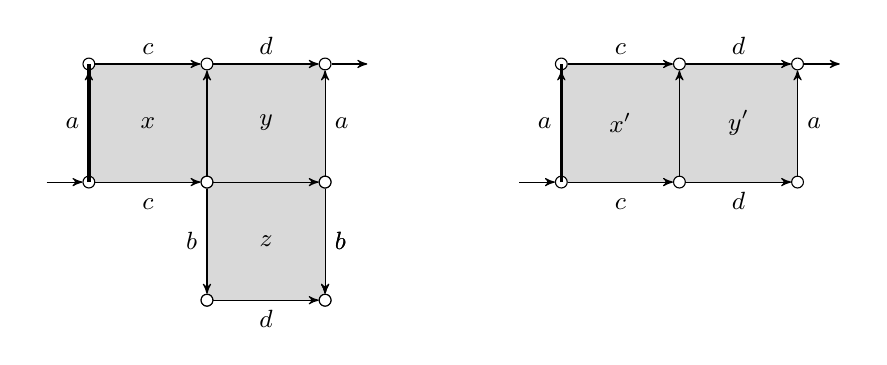
\begin{tikzpicture}[x=1.5cm, y=1.5cm]
  \begin{scope}[shift={(-2,0)}]
        \path[fill=black!15] (0,0) to (2,0) to (2,1) to (1,1) to
      (0,1);
      %%%%%
        \path[fill=black!15] (2,0) to (2,-1) to (1,-1) to
      (1,0);
      \node[state] (20) at (2,0) {};
      \node[state] (2-1) at (2,-1) {};
      \path (20) edge node[right] {$b$} (2-1);
      \node[state] (1-1) at (1,-1) {};
      \node[state] (10) at (1,0) {};
      \path (10) edge node[left] {$b$} (1-1);
      \path (20) edge node[right] {$b$} (2-1);
      \node[state] (2-1) at (2,-1) {};
      \node[state] (1-1) at (1,-1) {};
      \path (1-1) edge node[below] {$d$} (2-1);
       %\node (-.50) at (-.5,0) {$y_0$};% initial cell
      %%%%%
      \node[state, initial] (00) at (0,0) {};
      \node[state] (10) at (1,0) {};
      \node[state] (20) at (2,0) {};
      \node[state] (01) at (0,1) {};
      \node[state] (11) at (1,1) {};
      \node[state, accepting] (21) at (2,1) {};
      \path (00) edge node[below] {$\vphantom{d}c$} (10);
      \path (10) edge node[below] {} (20);
      \path (01) edge node[above] {$c$} (11);
      \path (11) edge node[above] {$d$} (21);
      \path (00) edge node[left] {$a$} (01);
      \path (10) edge (11);
      \path (20) edge node[right] {$a$} (21);
      %%%% cells names
      \node (.5.5) at (.5,.5) {$x$};
      \node (1.5.5) at (1.5,.5) {$y$};
      \node (1.5-.5) at (1.5,-.5) {$z$};
      
      \draw[-, very thick, black] (0,0) -- (0,1) ;
      \end{scope}

\begin{scope}[shift={(2,0)}]
        \path[fill=black!15] (0,0) to (2,0) to (2,1) to (1,1) to
      (0,1);
       % \node (-.50) at (-.5,0) {$z_0$};% initial cell
      %%%%%
      %%%%%
      \node[state, initial] (00) at (0,0) {};
      \node[state] (10) at (1,0) {};
      \node[state] (20) at (2,0) {};
      \node[state] (01) at (0,1) {};
      \node[state] (11) at (1,1) {};
      \node[state, accepting] (21) at (2,1) {};
      \path (00) edge node[below] {$\vphantom{d}c$} (10);
      \path (10) edge node[below] {$d$} (20);
      \path (01) edge node[above] {$c$} (11);
      \path (11) edge node[above] {$d$} (21);
      \path (00) edge node[left] {$a$} (01);
      \path (10) edge (11);
      \path (20) edge node[right] {$a$} (21);
      %% cells names
      \node (.5.5) at (.5,.5) {$x'$};
      \node (1.5.5) at (1.5,.5) {$y'$};
      \draw[-, very thick, black] (0,0) -- (0,1) ;
      \end{scope}


      
     %   \draw[-, very thick, red] (0,0) -- (1,0) -- (1,.5) -- 
% (1.5,.5) -- (1.5,1)  -- (2,1);
  %\node at (1.3,.7) {$\vphantom{b} \textcolor{red}{\alpha_1}$};
  %    \node[font=\normalsize] at (1,-.6) {$\pomset{ & a \\ c\ar[r]\ar[ur] & d}$};
  %      \node[font=\normalsize] at (1,-.9) {$c^+ c^-  a^+ d^+ a^- d^-  $};
  \end{tikzpicture}
   \smallskip
  \caption{Two $\TrO^0$-track bisimilar and not $\overline{\mathcal{U}}$-bisimilar HDAs.}
  \label{fig: counterexample }
\end{figure}

\begin{example}
   
 Fig \ref{fig: counterexample } shows two HDAs $(X,\{\delta_a^0(x)\},\{\delta^1_{ad}(y), \delta^1_{db}(z)\} )$ (on the left) and $(X',\{\delta_a^0(x')\},\{\delta^1_{ad}(y')\} )$ (on the right) that are $\TrO^0$-track bisimilar but not $\overline{\mathcal{U}}$-bisimular.  Let $P_1=\!\!\ipomset{\ar[r] & a  \ar@{.>}[d]  \ar[r]& 
      \\ & c  &}$, $P_2=\!\!\ipomset{\ar[r]  & a \ar@{.>}[d]
      \\ & d \ar[r] &}$, $P_3=\!\!\ipomset{ \ar[r] &  d \ar@{.>}[d]
      \\ & b &}$.
      It is not difficult to check that $K=\{(g,g')\mid g:\pobj{P} \to X,g':\pobj{P} \to X', P \stackrel{0}{\hookrightarrow} P_1*P_2  \}$ is a $\TrO^0$-track bisimulation. However, they cannot be $\overline{\mathcal{U}}$-bisimilar, because if there is a $\overline{\mathcal{U}}$-bisimulation between them, then $\delta^0_a(y)$ and $\delta^0_a(y')$ are related. However, $\delta_b^0(z)=\delta^0_a(y)$ while there exists no cell $z' \in X'$ such that $\delta_b^0(z')=\delta^0_a(y')$.  %$K=\bigl\{(g_{\alpha},g'_{\alpha'}) \mid (\alpha,\alpha')\in \{((\delta_a^0(x),x),(\delta_a^0(x'),x')),(y,y'), (z,z')\}  \bigl\}$
\end{example}
The following notion of behavioral equivalence is originally introduced by Van Glabbeek \cite{VANGLABBEEK2006265} as ST-bisimulaion. In our setting it has been formulated in \cite{VANGLABBEEK2006265} as follows.
 \begin{definition} \label{def: U bisimulation}
 A \emph{$\mathcal{U}$-bisimulation} between HDAs $\mathcal{Y}$ and $\mathcal{Z}$ is a relation $R$ between paths in $Y$ and $Z$ such that
\begin{enumerate}
\item \label{en: U bisim.e1} for any initial path $(y)$ where $ y\in I_Y$, $\emptyset \neq \{\alpha \in P_Z \mid ((y),\alpha) \in R \} \subseteq \{(z)\mid z \in I_Z \}$ and vice versa;%all initial paths $(y)$, where $ y\in I_Y $, are related to an initial path $(z)$ where $ z \in I_Z$ and vice-versa;
% $R$ is a bijection between initial unit paths $\{ (x); x\in I_Y \}$ and $\{ (y); y \in I_Z \}$;
%\item \label{en: U bisim.e2} $R$ respects final cells: for all
 % $( \rho, \sigma)\in R$, $end(\rho)\in F_X$ iff $end(\sigma) \in F_Y$;
\item \label{en: U bisim.e3} $R$ respects the shape: for all
  $( \rho, \sigma)\in R$, $\rho$ and $ \sigma$ have the same shape;
\item \label{en: U bisim.e4} for all $( \rho, \sigma)\in R$ and path
  $\rho'$ in $Y$ such that $\rho$ and $\rho'$ may be concatenated,
  there exists a path $\sigma'$ in $Z$ such that $( \rho * \rho',
  \sigma* \sigma')\in R$;
\item \label{en: U bisim.e5} for all $( \rho, \sigma)\in R$ and path
  $\sigma'$ in $Z$ such that $\sigma$ and $\sigma'$ may be
  concatenated, there exists a path $\rho'$ in $Y$ such that
  $( \rho* \rho', \sigma* \sigma')\in R$. %Whenever a path in $X$ can be extended, a related extension is available in $Y$ and vice versa. 
  
  A $\mathcal{U}$-bisimulation is called strong if, in addition, it satisfies:
\item \label{en: U bisim.e6} for all $( \rho, \sigma)\in R$ and $\rho'$ a restriction of $\rho$, there exists $\sigma'$ a restriction of $\sigma$ such that $( \rho',\sigma')\in R$.
\end{enumerate}
%A (strong) $\mathcal{U}$-bisimulation is called maximal if all paths in $Y$ are related to a path in $Z$ and vice-versa.
Finally, $\mathcal{X}$ and $\mathcal{Y}$ are (strong) \emph{$\mathcal{U}$-bisimilar} if there exists a (strong) $\mathcal{U}$-bisimulation $R$ between them; this is an equivalence relation.
\end{definition}

\begin{theorem}
   Two HDAs $\mathcal{X}_1$ and $\mathcal{X}_2$ are (strong) $T^0$-track bisimilar iff they are (strong) $\mathcal{U}$-bisimilar.
\end{theorem}
\begin{proof}
    $\Rightarrow$ Assume that there is a strong $\TrO^0$-track bisimulation $K$ between $\mathcal{X}_1$ and $\mathcal{X}_2$. We show that the relation between tracks with domain $\square^P$ given by $R=\{\bigl(p_1(\rho_P),p_2(\rho_P)\bigl) \mid (p_1,p_2)\in K\}$, where $\rho_P$ is the characteristic path of $P$, is a $\mathcal{U}$-bisimulation. By Yoneda lemma, there is a one-to-one correspondence between initial cells and initial tracks, thus $R$ satisfies \ref{def: U bisimulation}.\ref{en: U bisim.e1}. Since $p_i$ are precubical maps, \ref{def: U bisimulation}.\ref{en: U bisim.e3} is satisfied. Now to show \ref{def: U bisimulation}.\ref{en: U bisim.e4} and similarly \ref{def: U bisimulation}.\ref{en: U bisim.e5}, let $(\alpha_1,\alpha_2)\in R$ so that $(\alpha_1,\alpha_2)=\bigl(p_1(\rho_P),p_2(\rho_P)\bigl)$ for some $(p_1,p_2)\in K$. Assume that there exists $\beta_2$ such that $\alpha_1$ and $\beta_2$ can be concatenated in $X_1$. Let $Q=P*R=\ev(\alpha*\beta)$ and $\rho_Q$ the characteristic path of $Q$. By Proposition \ref{prop: prop: generalization of yoneda }, there exists a track $p'_1: \square^Q \to X_1$ such that $p'_1(\rho_Q)=\alpha*\beta=p_1(\rho_P)*\beta$. On the other hand, by definition \ref{def: char path}, we have $\rho_Q=\jneda^0_{P\subseteq Q}*\rho$ for some $\rho \in P_{\pobj{Q}}$). Thus $p'_1(\rho_Q)=p'_1(\jneda^0_{P\subseteq Q}*\rho)$, therefore by identification, $p'_1 \circ \jneda^0_{P\subseteq Q}(\rho_P)=p_1(\rho_P)$. By the generalization of Yoneda Lemma (Proposition \ref{prop: prop: generalization of yoneda }), $p'_1 \circ \jneda^0_{P\subseteq Q}=p_1$. By the property \ref{def: track bisimulation}.\ref{eq2: track bis} satisfied by $K$, there exists $p'_2:\square^Q \to Z$ such that $(p'_1,p'_2) \in K$ and $p'_2 \circ \jneda^0_{R\subseteq Q}=p_2$. Defining $\beta_2= p'_2(\rho)$, we obtain $p'_2(\rho_Q)=\alpha_2*\beta_2$, meaning that $\alpha_2$ can be concatenated with $\beta_2$, and see $(\alpha_1*\beta_1,\alpha_2*\beta_2) \in K$. Finally, $K$ is strong since $R$ is strong.

    $\Leftarrow$ For any path $\alpha \in \mathrm{P}_{X}$, we denote by $p_{\alpha}: \pobj{\ev(\alpha)} \to X$ the track of proposition \ref{prop: prop: generalization of yoneda }. We assume that there is a strong $\mathcal{U}$-bisimulation $R$ between HDAs $\mathcal{X}_1$ and $\mathcal{X}_2$. We show that the relation between tracks $K=\{(p_{\alpha_1},p_{\alpha_2})\mid (\alpha_1,\alpha_2) \in K \}$ is a strong $\TrO^0$-bisimulation. First, $K$ satisfies \ref{def: track bisimulation}.\ref{eq1: track bis} because there is one-to-one correspondence between initial tracks and initial cells (Yoneda embedding). To show \ref{def: track bisimulation}.\ref{eq2: track bis}, let $(p_{\alpha_1},p_{\alpha_2}) \in K$. Assume that there exists a track $p'_1:\pobj{Q} \to X_1 $, where $P=\ev(\alpha_1)=\ev(\alpha_2)$ and $P \ininc Q$, such that $p'_1 \circ \jneda^0_{P\subseteq Q}=p_{\alpha_1}$. Let $\rho_Q$ the characteristic path of $Q$. By definition \ref{def: char path} of $\rho_Q$ then by proposition \ref{prop: prop: generalization of yoneda }, $p'_1(\rho_Q)=(p'_1 \circ \jneda^0_{P\subseteq Q})(\rho_P)*\beta_1= \alpha_1*\beta_1$ for some $\beta_1 \in P_{X_1}$. That is, $\alpha_1$ can be concatenated with some $\beta_1$, thus by \ref{def: U bisimulation}.\ref{en: U bisim.e4}, $\alpha_2$ can be concatenated with some $\beta_2 \in P_{X_2}$ such that $(\alpha_1*\beta_1,\alpha_2*\beta_2) \in R$. Defining $p_2'=p_{\alpha_2*\beta_2}$, we obtain $(p'_1,p'_2)\in K$ and we can check that $p'_2 \circ \jneda^0_{P\subseteq Q}=p_{\alpha_2}$ again by Proposition \ref{prop: prop: generalization of yoneda } and the Definition \ref{def: char path} of the characteristic path. Finally, it is not difficult to check that if $R$ is strong, then $K$ is strong.
\end{proof}





%\begin{theorem}
%    The following are equivalent:
%       \begin{enumerate}
%        \item $\mathcal{Y}$ and $\mathcal{Z}$ are strong $\mathcal{U}$-bisimilar,
%        \item $\mathcal{Y}$ and $\mathcal{Z}$ are strong $\TrO^0$-track bisimular.
%    \end{enumerate}
%\end{theorem}


%\paragraph*{Conclusion}
%We introduced a notion of bisimulation between cells of HDAs, namely $\overline{\mathcal{U}}$-bisimulation. We considered $T^0$ as the subcategory of track objects as objects and morphisms are initial inclusions and showed that $\overline{\mathcal{U}}$-bisimularity is equivalent to having a span of $T^0$-open maps ($T^0$-bisimularity), that is, maps that have the future path lifting property. Finally, we constructed a Hennessey-Milner logic interpreted over HDAs and that characterizes $\overline{\mathcal{U}}$-bisimulation.
\vspace{1cm}

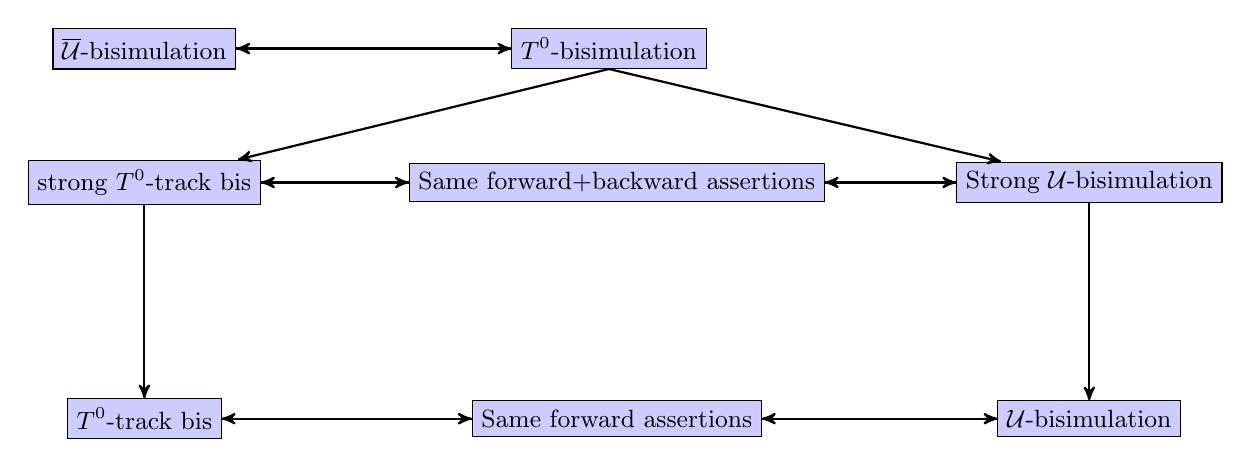
\begin{tikzpicture}[fill=blue!20] 
%\caption{test}
%\draw[help lines] (-1,-2) grid (6,3);
\path (1.6,3.2) node(ubar) [rectangle,rotate=0,draw,fill] {$\overline{\mathcal{U}}$-bisimulation}
(1.6,1.5) node(strong_t0_track) [rectangle,draw,fill] { strong $T^0$-track bis }
(1.6,-1.5) node(t0_track) [rectangle,draw,fill] {$T^0$-track bis }
(13.6,1.5) node(strong_U_bis) [rectangle,draw,fill] { Strong $\mathcal{U}$-bisimulation}
(13.6,-1.5) node(U_bis) [rectangle,draw,fill] { $\mathcal{U}$-bisimulation}
(7.6,1.5) node(all_asssertions) [rectangle,rotate=0,draw,fill] {Same forward+backward assertions}
(7.6,-1.5) node(asssertions) [rectangle,rotate=0,draw,fill] {Same forward assertions}
(7.5,3.2) node(t0bis) [rectangle,rotate=-0,draw,fill] {$T^0$-bisimulation};
%(3,3.2) node(aa) [rectangle,rotate=-0,draw,fill] { $\overline{\mathcal{U}}$-bisimulation};


%(3.2,2) node(c) [rectangle,rotate=0,draw,fill] {Bisimulation involving homotopy}
%\draw[thick] (a.south) -- (c);
\draw[thick] (strong_t0_track) -- (all_asssertions);
\draw[thick] (all_asssertions) -- (strong_t0_track);
\draw[thick]  (strong_t0_track) -- (t0_track) ;

\draw[thick] (t0bis) -- (ubar);
\draw[thick] (ubar) -- (t0bis);

\draw[thick] (t0_track) -- (asssertions);
\draw[thick] (asssertions) -- (t0_track);
%\draw[thick] (a.south) -- (e);
%\draw[thick] (b) -- (ubar);
%\draw[thick] (ubar) -- (b);
%\draw[thick] (d.south) -- (e);
%\draw[thick] (d)  -- (ubar);
%\draw[thick] (ubar)  -- (d);
\draw[thick] (t0bis.south) -- (strong_t0_track);
\draw[thick] (t0bis.south) -- (strong_U_bis);
\draw[thick] (strong_U_bis) -- (U_bis);
\draw[thick] (strong_U_bis) --  (all_asssertions) ;
\draw[thick] (all_asssertions) -- (strong_U_bis);
\draw[thick] (U_bis) --  (asssertions) ;
\draw[thick] (asssertions) -- (U_bis);
%\draw[thick] (d) -- (t0bis.south);
%\draw[thick] (ubar)  -- (e);
%\draw[thick,red,->] (a) \mid- +(1,3) -\mid (c) \mid- (b);
%\draw[thick,blue,<->] (b) .. controls +(right:2cm) and +(down:1cm) .. (d);
\end{tikzpicture}

\subsection{Characterisation of hh-bisimulation}



\appendix

\chapter{Additional}



\bibliographystyle{unsrt}
\bibliography{sample}

\end{document}

